\documentclass[11pt,twoside,a4paper]{article}
% http://www-h.eng.cam.ac.uk/help/tpl/textprocessing/latex_maths+pix/node6.html symboles de math
% http://fr.wikibooks.org/wiki/Programmation_LaTeX Programmation latex (wikibook)
%=========================== En-Tete =================================
%--- Insertion de paquetages (optionnel) ---
\usepackage[french]{babel}   % pour dire que le texte est en fran{\'e}ais
\usepackage{a4}	             % pour la taille   
\usepackage[T1]{fontenc}     % pour les font postscript
\usepackage{epsfig}          % pour gerer les images
%\usepackage{psfig}
\usepackage{amsmath, amsthm} % tres bon mode mathematique
\usepackage{amsfonts,amssymb}% permet la definition des ensembles
\usepackage{float}           % pour le placement des figure
\usepackage{verbatim}

\usepackage{longtable} % pour les tableaux de plusieurs pages

\usepackage[table]{xcolor} % couleur de fond des cellules de tableaux

\usepackage{lastpage}

\usepackage{multirow}

\usepackage{multicol} % pour {\'e}crire dans certaines zones en colonnes : \begin{multicols}{nb colonnes}...\end{multicols} 

% \usepackage[top=1.5cm, bottom=1.5cm, left=1.5cm, right=1.5cm]{geometry}
% gauche, haut, droite, bas, entete, ente2txt, pied, txt2pied
\usepackage{vmargin}
\setmarginsrb{1.0cm}{1.0cm}{1.0cm}{1.0cm}{15pt}{3pt}{57pt}{25pt}

\usepackage{lscape} % changement orientation page
%\usepackage{frbib} % enlever pour obtenir references en anglais
% --- style de page (pour les en-tete) ---
\pagestyle{headings}

\def\MainTitle{Bitcoin : Quelques articles...}

% % % en-tete et pieds de page configurables : fancyhdr.sty

% http://www.trustonme.net/didactels/250.html

% http://ww3.ac-poitiers.fr/math/tex/pratique/entete/entete.htm
% http://www.ctan.org/tex-archive/macros/latex/contrib/fancyhdr/fancyhdr.pdf
\usepackage{fancyhdr}
\pagestyle{fancy}
% \newcommand{\chaptermark}[1]{\markboth{#1}{}}
% \newcommand{\sectionmark}[1]{\markright{\thesection\ #1}}
\fancyhf{}
\fancyhead[LE,RO]{\bfseries\thepage}
\fancyhead[LO]{\bfseries\rightmark}
\fancyhead[RE]{\bfseries\leftmark}
\fancyfoot[LE]{\thepage /\pageref{LastPage} \hfill
	\MainTitle 
\hfill 
\includegraphics[width=0.5cm]{img/logo_glider.png} }
\fancyfoot[RO]{
\includegraphics[width=0.5cm]{img/logo_glider.png} \hfill
	\MainTitle 
\hfill \thepage /\pageref{LastPage}}
\renewcommand{\headrulewidth}{0.25pt}
\renewcommand{\footrulewidth}{0.50pt}
\addtolength{\headheight}{0.5pt}
\fancypagestyle{plain}{
	\fancyhead{}
	\renewcommand{\headrulewidth}{0pt}
}

%--- Definitions de nouvelles commandes ---
\newcommand{\N}{\mathbb{N}} % les entiers naturels

%--- Definitions de nouvelles couleurs ---
\definecolor{verylightgrey}{rgb}{0.8,0.8,0.8}
\definecolor{verylightgray}{gray}{0.80}
\definecolor{lightgrey}{rgb}{0.6,0.6,0.6}
\definecolor{lightgray}{gray}{0.6}

\usepackage{lettrine}
\usepackage{fancybox}
\usepackage{textcomp} %% euro, florin...
\usepackage{eurosym}

%============================= Corps =================================
\begin{document}

\setlength\parindent{0pt}

%% \texttt{  }~\\

%% \textbf{\LARGE }~\\

%% \emph{\small }~\\

%% \begin{minipage}[ht]{0.75\textwidth}
%% 	~\\
%% \end{minipage} \hfill \begin{minipage}[ht]{6.15cm}
%% 	\includegraphics[width=6.00cm]{img/*****}
%% \end{minipage}~\\~\\

%% \clearpage

\texttt{http://www.lemonde.fr/technologies/article/2011/06/17/bitcoin-les-deux-faces-de-la-monnaie-virtuelle\_1537285\_651865.html}~\\

\textbf{Bitcoin, les deux faces de la monnaie virtuelle}~\\

\textbf{\small \emph{Par Laurent Checola} | Le Monde.fr | 17.06.2011 {\`a} 14h03 -- Mis {\`a} jour le 17.06.2011 {\`a} 15h05  }~\\

\begin{minipage}[ht]{6.25cm}	
	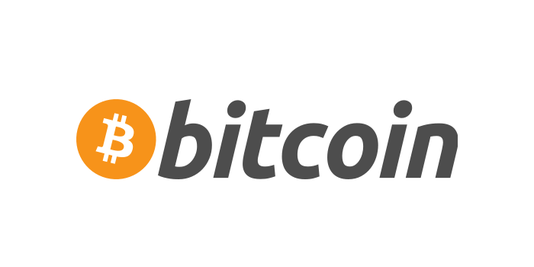
\includegraphics[width=6.00cm]{img/1537310_3_ab4d_le-logo-de-la-monnaie-virtuelle-bitcoin.png} ~\\
	\emph{Le logo de la monnaie virtuelle bitcoin. | Bitcoin}
\end{minipage} \hfill \begin{minipage}[ht]{12.50cm}
	"\emph{Un mod{\`e}le de paiement {\'e}lectronique de pair {\`a} pair, permettant d'envoyer directement de l'argent d'une personne {\`a} une autre, sans passer par une institution financi{\`e}re.}" C'est ainsi que Satoshi Nakamoto, le myst{\'e}rieux inventeur des "bitcoins", \texttt{d{\'e}crit son invention~\footnotemark}. ~\\
	
	Ce syst{\`e}me, qui permet d'{\'e}changer en ligne de l'argent de mani{\`e}re d{\'e}centralis{\'e}e, existe depuis 2009. Mais la "valeur" du bitcoin sur les plates-formes d'{\'e}changes a consid{\'e}rablement augment{\'e} ces derni{\`e}res semaines, chaque "pi{\`e}ce virtuelle" passant au-dessus des 20 dollars (14 euros). Pour pouvoir {\'e}changer des bitcoins, les internautes doivent installer un logiciel sur leur ordinateur. Ces utilisateurs allouent d{\`e}s lors une partie de la capacit{\'e} de calcul de leur ordinateur, et contribuent au processus de s{\'e}curisation des transactions. ~\\
\end{minipage}~\\
~\footnotetext{\texttt{http://www.bitcoin.org/bitcoin.pdf}}

\textbf{\textsc{R{\'E}SISTANCE {\`A} L'INFLATION}}~\\

Ce syst{\`e}me permet {\'e}galement de g{\'e}n{\'e}rer, au compte-gouttes, de nouveaux bitcoins, un algorithme gratifiant au hasard un internaute pour sa contribution. Au total, Satoshi Nakamoto a pr{\'e}vu qu'environ 21 millions de bitcoins devraient {\^e}tre {\'e}mis d'ici 2030, selon une courbe pr{\'e}visible. "\emph{Par certains aspects, le bitcoin ressemble {\`a} des monnaies comme l'or car il y a une masse globale connue en circulation. Elle r{\'e}siste donc {\`a} l'inflation et sa stabilit{\'e} ne d{\'e}pend pas d'un pays en particulier. Mais le bitcoin ressemble aussi {\`a} de la monnaie fiduciaire. Comme l'euro par exemple, la valeur d'un bitcoin d{\'e}pend du fait que certaines personnes sont pr{\^e}tes {\`a} l'accepter comme un moyen de paiement pour les biens et services}", analyse Vili Lehdonvirta, sp{\'e}cialiste des biens virtuels et auteur d'une {\'e}tude pour la Banque mondiale. ~\\

Outre la "\emph{g{\'e}n{\'e}ration spontan{\'e}e}" de cette monnaie virtuelle, des plates-formes permettent de r{\'e}aliser des {\'e}changes contre des dollars ou des euros. C'est le cas de sites comme \texttt{Mt. Gox Bitcoin Exchange\footnote{\texttt{https://mtgox.com/}} } ou \texttt{BitMarket.eu\footnote{\texttt{https://bitmarket.eu/}} }. "\emph{{\'E}tant donn{\'e} que l'offre de bitcoins est relativement stable, la r{\'e}cente demande, fruit de l'attention des m{\'e}dias, a naturellement augment{\'e} son prix. Mais si cet int{\'e}r{\^e}t se dissipe, la valeur pourrait faire de m{\^e}me}", pr{\'e}vient Vili Lehdonvirta. --- Ce n'est pas la premi{\`e}re fois que des monnaies virtuelles tentent de conqu{\'e}rir le Web. D{\`e}s la fin des ann{\'e}es 1990, des devises comme Flooz, Beenz, les Linden dollars ou l'e-gold avaient tent{\'e} de percer. "\emph{Contrairement {\`a} d'autres devises d{\'e}centralis{\'e}es, un contr{\^o}le de fer est exerc{\'e} sur l'offre et sur les transactions effectu{\'e}es}", pr{\'e}cise l'expert des biens virtuels. ~\\

\textbf{\textsc{TRANSACTIONS DIFFICILES {\`A} R{\'E}GULER}}~\\

Pour l'utilisateur de bitcoins, "\emph{l'une des raisons de l'adoption est le faible co{\^u}t pr{\'e}lev{\'e} sur les transactions. Mais une autre raison importante est que les transactions peuvent {\^e}tre r{\'e}alis{\'e}es anonymement, sans contr{\^o}le possible des services fiscaux}", analyse M. Lehdonvirta. --- Outre des experts des biens virtuels, qui pointent la difficult{\'e} {\`a} r{\'e}guler le syst{\`e}me, certains politiques s'inqui{\`e}tent aussi des potentiels usages des bitcoins. Une liste de plus en plus longue de sites Web, proposant des services ou des produits, acceptent cette monnaie. Mais aux Etats-Unis, deux s{\'e}nateurs d{\'e}mocrates, Charles Schumer, de New York, et Joe Manchin, de Virginie-Occidentale, ont demand{\'e}, au d{\'e}but du mois de juin {\`a} l'Etat f{\'e}d{\'e}ral de mettre fin {\`a} un dispositif qui \texttt{encouragerait le blanchiment d'argent\footnote{\texttt{http://terranova.blogs.com/terra\_nova/2011/06/a-bit-too-far.html}} }. Sans compter que ce syst{\`e}me d{\'e}centralis{\'e} {\`a} l'extr{\^e}me pose des questions \texttt{sur les recours disponibles\footnote{\texttt{http://arstechnica.com/tech-policy/news/2011/06/bitcoin-the-decentralized-virtual-currencyrisky-currency-500000-bitcoin-heist-raises-questions.ars}} } pour un utilisateur victime d'un vol ou d'une escroquerie. Sur Twitter, le groupe de pirates informatiques LulzSec expliquait avoir re\c{c}u 7 200 dollars (5 000 euros) en bitcoins, et le site AnonOps, li{\'e} {\`a} Anonymous, accepte d{\'e}sormais ce type de cr{\'e}dits virtuels. ~\\

"\emph{Il sera tr{\`e}s difficile de r{\'e}guler les transactions effectu{\'e}es en bitcoins. C'est comme l'{\'e}change de fichiers en peer-to-peer : pour le r{\'e}guler, il faut souvent des lois intrusives, qui menacent la vie priv{\'e}e et la libert{\'e} d'expression"}, pr{\'e}vient Vili Lehdonvirta. L'expert voit toutefois dans les plates-formes d'{\'e}changes comme Mt. Gox un maillon un peu plus faible dans la cha{\^i}ne de l'anonymat des transactions. ~\\

Et si Bitcoin se passe d'une entreprise tierce pour assurer la validit{\'e} des transactions, les g{\'e}ants du paiement en ligne, comme Visa, Mastercard ou Paypal, semblent pour l'heure peu menac{\'e}s. "\emph{Pour l'instant, le syst{\`e}me Bitcoin est trop difficile {\`a} prendre en main par l'utilisateur moyen et ne menace donc pas les syst{\`e}mes de paiement les plus connus}", note M. Lehdonvirta. %% ~\\

%% \emph{Laurent Checola}~\\

\dotfill %% \clearpage

\texttt{http://www.lemonde.fr/technologies/article/2011/06/20/la-monnaie-virtuelle-bitcoin-en-crise\_1538194\_651865.html}~\\

\textbf{La monnaie virtuelle bitcoin en crise}~\\

\textbf{\small Le Monde.fr | 20.06.2011 {\`a} 12h42 -- Mis {\`a} jour le 20.06.2011 {\`a} 13h35 }~\\

\begin{minipage}[ht]{6.25cm}	
	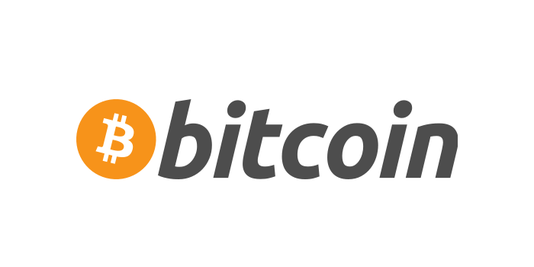
\includegraphics[width=6.00cm]{img/1537310_3_ab4d_le-logo-de-la-monnaie-virtuelle-bitcoin.png} ~\\
	\emph{Le logo de la monnaie virtuelle bitcoin. | Bitcoin}
\end{minipage} \hfill \begin{minipage}[ht]{12.50cm}
	La valeur de la monnaie virtuelle d{\'e}centralis{\'e}e bitcoin est-elle en train de s'effondrer ? Sur la plate-forme d'{\'e}changes Mt. Gox, \texttt{la valeur du bitcoin\footnotemark} a brutalement chut{\'e}, dimanche 19 juin, passant en quelques heures d'environ 17 dollars (12 euros) {\`a} pr{\`e}s de z{\'e}ro. Cet effondrement du cours intervient apr{\`e}s l'apparition d'une faille dans la s{\'e}curit{\'e} du site Mt. Gox, exposant les donn{\'e}es de milliers de ses utilisateurs. ~\\
	
	La monnaie bitcoin, cr{\'e}{\'e}e en 2009, fait l'objet de l'attention des m{\'e}dias depuis quelques semaines. Le syst{\`e}me des bitcoins offre notamment la possibilit{\'e} d'{\'e}changer en ligne de l'argent de mani{\`e}re d{\'e}centralis{\'e}e, de pair {\`a} pair, sans intervention d'une entreprise tierce pour s{\'e}curiser les transactions. Il permet {\'e}galement d'acheter directement sur divers sites Web un certain nombre de produits, pay{\'e}s en monnaie virtuelle. ~\\
\end{minipage}~\\
\footnotetext{\texttt{http://leanback.eu/bitcoin/plots/20110619195756-mtgox.png}}

Par ailleurs, le syst{\`e}me pr{\'e}sente l'originalit{\'e} de g{\'e}n{\'e}rer de nouveaux bitcoins selon une courbe pr{\'e}visible par un algorithme. Dans ce dispositif, plusieurs plates-formes comme Mt. Gox sont apparues, qui font office de guichet de change bitcoins-dollars. ~\\

\textbf{\textsc{PROBL{\`E}ME GLOBAL ?}}~\\

Dans un \texttt{communiqu{\'e}\footnote{\texttt{https://support.mtgox.com/entries/20208066-huge-bitcoin-sell-off-due-to-a-compromised-account-rollback}}}, Mt. Gox annonce avoir ferm{\'e} sa plate-forme jusqu'{\`a} ce que le probl{\`e}me soit r{\'e}solu. Mais, depuis l'annonce du piratage, les donn{\'e}es incluant le nom et l'adresse email de milliers d'utilisateurs circulent n{\'e}anmoins sur le Web. Mt. Gox invite d{\`e}s lors les utilisateurs {\`a} changer de mot de passe. Ce n'est pas la premi{\`e}re fois que la s{\'e}curit{\'e} des transactions impliquant les bitcoins est mise en cause. La semaine derni{\`e}re, un utilisateur s'est dit \texttt{victime d'une escroquerie\footnote{\texttt{http://forum.bitcoin.org/index.php?topic=16457.0}}} qui lui aurait fait perdre 25 000 bitcoins. --- Si la baisse de la valeur sur Mt. Gox est spectaculaire, elle ne semble pas paradoxalement mettre en p{\'e}ril la s{\'e}curit{\'e} globale du syst{\`e}me bitcoin. Les plates-formes d'{\'e}change comme Mt. Gox constituent en effet le maillon le plus faible dans la cha{\^i}ne de l'anonymat des transactions. Sur des \texttt{sites concurrents\footnote{\texttt{https://www.tradehill.com/MarketData/}}} de Mt. Gox, comme Tradehill, la valeur du bitcoin est d'ailleurs demeur{\'e}e plut{\^o}t stable. ~\\

\clearpage

\texttt{http://www.lemonde.fr/sciences/article/2012/11/29/payer-et-vendre-sans-les-banques\_1798066\_1650684.html}~\\

\textbf{Avec Bitcoin, payer et vendre sans les banques}~\\

\textbf{\small \emph{Par David Larousserie} LE MONDE SCIENCE ET TECHNO | 29.11.2012 {\`a} 16h12 -- Mis {\`a} jour le 01.12.2012 {\`a} 18h23 }~\\

Wordpress va accepter le syst{\`e}me de monnaie bitcoin, \texttt{a annonc{\'e}\footnote{\texttt{http://en.blog.wordpress.com/2012/11/15/pay-another-way-bitcoin/}} }, jeudi 15 novembre, la plateforme de blogs. Worpress, plateforme \emph{open source}, est disponible gratuitement pour les utilisateurs, qui peuvent toutefois ajouter de nouvelles fonctionnalit{\'e}s, payantes. ~\\

"\emph{Un service comme Paypal emp{\^e}che les paiements de plus de 60 pays et de nombreux services bancaires appliquent des restrictions similaires}", justifie Wordpress. D'apr{\`e}s les \texttt{statistiques de l'h{\'e}bergeur\footnote{\texttt{http://en.wordpress.com/stats/}}}, pr{\`e}s de 58 millions de sites dans le monde utilisent Wordpress. ~\\

\textbf{\textsc{MONNAIE D{\'E}CENTRALIS{\'E}E}}~\\

La monnaie bitcoin a {\'e}t{\'e} cr{\'e}{\'e}e en 2009, sa principale caract{\'e}ristique {\'e}tant la possibilit{\'e} d'{\'e}changer en ligne de l'argent de mani{\`e}re d{\'e}centralis{\'e}e, de pair {\`a} pair, sans intervention d'une entreprise tierce. Le syst{\`e}me g{\'e}n{\`e}re aussi de nouveaux bitcoins selon une courbe pr{\'e}visible par un algorithme. Dans ce dispositif, plusieurs plateformes comme Mt. Gox sont apparues, qui font office de guichet de change bitcoins-dollars. ~\\

Si cette monnaie virtuelle a suscit{\'e} l'int{\'e}r{\^e}t des m{\'e}dias en 2011, elle a aussi connu des rat{\'e}s. En juin 2011, la platefgorme Mt. Gox avait ainsi d{\^u} reconna{\^i}tre une importante \texttt{faille\footnote{\texttt{http://www.lemonde.fr/technologies/article/2011/06/20/la-monnaie-virtuelle-bitcoin-en-crise\_1538194\_651865.html}}} de s{\'e}curit{\'e}. Sur les plateformes d'{\'e}change, un bitcoin vaut d{\'e}sormais autour de 11 dollars (8,60 euros). ~\\


\clearpage

\texttt{http://www.lemonde.fr/technologies/article/2012/11/19/la-plateforme-wordpress-s-ouvre-au-bitcoin\_1792596\_651865.html}~\\

\textbf{La plateforme Wordpress s'ouvre au bitcoin}~\\

\textbf{\small Le Monde.fr | 19.11.2012 {\`a} 10h45 -- Mis {\`a} jour le 19.11.2012 {\`a} 11h16 }~\\

\begin{minipage}[ht]{6.25cm}	
	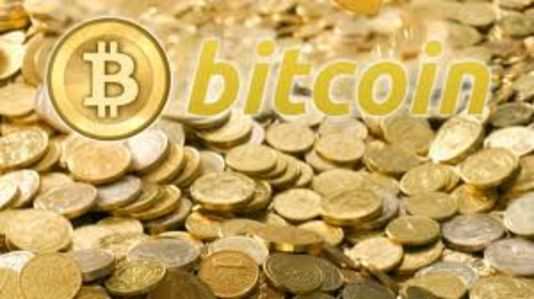
\includegraphics[width=6.00cm]{img/1798142_5_9dc4_le-systeme-de-monnaie-virtuelle-bitcoin_9f6a91df917eb587cc1841d336dfc7a5.jpg} ~\\
	\emph{Le syst{\`e}me de monnaie virtuelle bitcoin s'appuie sur un r{\'e}seau pair {\`a} pair pour {\'e}changer des unit{\'e}s de compte. | bitcoin}~\\
\end{minipage} \hfill \begin{minipage}[ht]{12.50cm}
	Internet continue de faire vaciller les bases des secteurs les plus {\'e}tablis : la musique, le cin{\'e}ma, le commerce, la presse. Et maintenant les banques ! Une technologie, \texttt{Bitcoin\footnotemark}, f{\^e}tera son quatri{\`e}me anniversaire en janvier 2013 avec la promesse de cr{\'e}er un r{\'e}seau de transactions financi{\`e}res d{\'e}centralis{\'e}, anonyme et sans frais. ~\\
	
	Tout le contraire des {\'e}changes mon{\'e}taires actuels, bas{\'e}s sur des banques centrales, des transactions identifi{\'e}es et des frais de traitement entre les parties prenantes. En outre, comme souvent dans ces technologies, une vision politique est palpable : la conviction que le syst{\`e}me mon{\'e}taire actuel, fait de monopoles bancaires, conduit aux crises financi{\`e}res. ~\\
\end{minipage}~\\
\footnotetext{\texttt{http://www.bitcoin.org/}}

En fait, Bitcoin, invent{\'e} par Satoshi Nakamoto (un pseudonyme), est {\`a} la fois une monnaie virtuelle (mais convertible en dollars, euros...) et un protocole d'{\'e}change s{\'e}curis{\'e} {\`a} la mani{\`e}re de BitTorrent, qui permet l'{\'e}change de fichiers de pair {\`a} pair. ~\\

Environ 200 000 transactions ont d{\'e}j{\`a} {\'e}t{\'e} enregistr{\'e}es gr{\^a}ce {\`a} 15 000 ordinateurs sur le r{\'e}seau. Un petit millier de sites Web acceptent les bitcoins comme dons ou comme moyen de paiement. Le cours du bitcoin, apr{\`e}s avoir atteint un sommet de 30 dollars (23 euros) en juin 2011, a chut{\'e} {\`a} 2 dollars, cinq mois plus tard, avant de revenir aujourd'hui autour d'une dizaine de dollars (les cours sont recens{\'e}s sur le site bitcoincharts. com). Rien de tr{\`e}s impressionnant, compar{\'e} aux {\'e}changes mondiaux en monnaie r{\'e}elle ou en produits financiers. ~\\

\begin{minipage}[ht]{6.25cm}	
	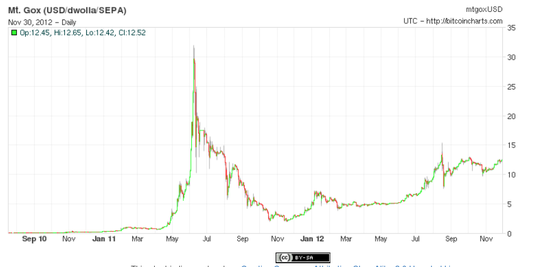
\includegraphics[width=6.00cm]{img/1798258_3_a2bb_les-fluctuations-de-la-valeur-en-dollars-du_3be730c4ac7d5cf3c9b859a1a8ca9d50.png} ~\\
	\emph{Les fluctuations de la valeur, en dollars, du Bitcoin sur l'une des plateformes les plus connues, Mt. Gox | Mt.Gox/bitcoincharts.com}~\\
\end{minipage} \hfill \begin{minipage}[ht]{12.50cm}
	Pourtant, la Banque centrale europ{\'e}enne (BCE) s'y est int{\'e}ress{\'e}e dans un \texttt{rapport sur les monnaies virtuelles publi{\'e} en octobre\footnotemark}. Elle d{\'e}crit bitcoin comme "\emph{la monnaie virtuelle ayant le plus de succ{\`e}s}", "\emph{en comp{\'e}tition avec le dollar ou l'euro}" et "\emph{similaire {\`a} des monnaies conventionnelles}". Bitcoin se distingue d'autres types de monnaie virtuelle comme les "cr{\'e}dits", utilis{\'e}s pour progresser dans un jeu vid{\'e}o que l'on gagne en jouant ou que l'on peut acheter (et parfois {\'e}changer en retour). ~\\
	
	Le r{\'e}seau social Facebook a aussi d{\'e}velopp{\'e} ce genre de syst{\`e}me. Mais, chaque fois, une autorit{\'e} centrale contr{\^o}le et traite les {\'e}changes. Avec Bitcoin, tous les noeuds du r{\'e}seau sont {\`a} la fois d{\'e}positaires du livre de comptes, v{\'e}rificateurs, {\'e}metteurs de monnaie, et acheteurs et vendeurs. ~\\
\end{minipage}~\\
\footnotetext{\texttt{http://www.ecb.int/pub/pdf/other/virtualcurrencyschemes201210en.pdf}}


Comment fonctionne ce r{\'e}seau ? Chaque transaction entre deux utilisateurs se fait en r{\'e}alit{\'e} entre deux adresses {\'e}lectroniques {\`a} la mani{\`e}re d'un e-mail. Sauf qu'un utilisateur peut choisir une adresse diff{\'e}rente pour chaque paiement, assurant ainsi l'anonymat. Un ensemble d'informations li{\'e}es {\`a} cette transaction est sign{\'e} {\'e}lectroniquement par un syst{\`e}me de chiffrement {\`a} double cl{\'e}. Le r{\'e}seau peut ainsi v{\'e}rifier l'authenticit{\'e} de la transaction. Gr{\^a}ce au contenu du fichier, il est aussi possible de s'assurer que les bitcoins {\'e}chang{\'e}s existent bien dans le livre de comptes public, diffus{\'e} dans tout le r{\'e}seau. ~\\

\begin{minipage}[ht]{6.25cm}	
	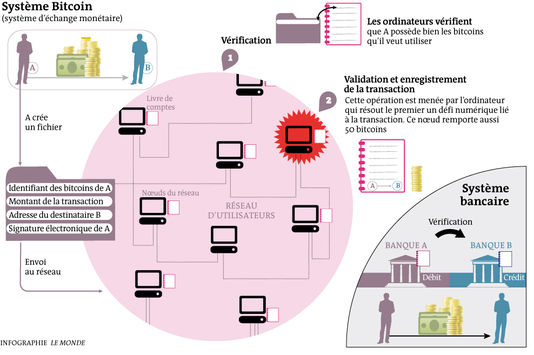
\includegraphics[width=6.00cm]{img/1798255_5_2076_le-systeme-d-echange-monetaire-bitcoin_f2e60fed9a4542a2589e1e9e6317fcdc.jpg} ~\\
	\emph{Le syst{\`e}me d'{\'e}change mon{\'e}taire Bitcoin. | Infographie Le Monde}~\\
\end{minipage} \hfill \begin{minipage}[ht]{12.50cm}
	L'{\'e}tape-cl{\'e} consiste {\`a} {\'e}crire cette nouvelle transaction dans ce livre. Elle passe par la r{\'e}solution d'un d{\'e}fi math{\'e}matique lanc{\'e} aux ordinateurs, et dont le gagnant, sorte de banquier central provisoire, aura le privil{\`e}ge d'ajouter cette ligne suppl{\'e}mentaire. Il s'agit d'une phase de hachage de fichier, c'est-{\`a}-dire de transformation d'un gros fichier en une empreinte num{\'e}rique plus courte et unique. Les ordinateurs "prennent" la nouvelle transaction et lui ajoutent un nombre avant de "hacher" l'ensemble. ~\\
	
	Le but {\'e}tant de trouver le nombre qui donne une empreinte particuli{\`e}re (beaucoup de z{\'e}ros au d{\'e}but). Une fois ce nombre trouv{\'e}, les autres noeuds v{\'e}rifient ais{\'e}ment que c'est le bon. La transaction se trouve alors indestructiblement li{\'e}e {\`a} la cha{\^i}ne de l'ensemble des autres transactions ; toute modification changerait l'empreinte. ~\\
\end{minipage}~\\

Si, pour frauder, un utilisateur voulait payer deux fois avec le m{\^e}me argent tr{\`e}s vite (moins de dix minutes), une seule des deux transactions serait valid{\'e}e par le r{\'e}seau -- l'autre restant orpheline car les deux ont des empreintes diff{\'e}rentes. L'ordinateur ayant r{\'e}solu le d{\'e}fi remporte 50 bitcoins. Pour {\'e}viter l'inflation, cette r{\'e}compense est divis{\'e}e par deux r{\'e}guli{\`e}rement, probablement avant la fin 2012. Le nombre de bitcoins en circulation est donc limit{\'e} {\`a} 21 millions, mais ils sont divisibles jusqu'au cent millioni{\`e}me, ce qui laisse de la marge... La difficult{\'e} du d{\'e}fi est aussi relev{\'e}e {\`a} chaque augmentation de la puissance de calcul. ~\\

La vie du r{\'e}seau a d{\'e}j{\`a} eu des hauts et des bas. Des sites Web fournissant des services pour Bitcoin ont {\'e}t{\'e} attaqu{\'e}s et les bitcoins en d{\'e}p{\^o}ts vol{\'e}s. "\emph{La faille utilis{\'e}e ne concerne pas le protocole lui-m{\^e}me}", assure Pierre Noizat, qui vient de lancer \texttt{Paymium\footnote{\texttt{http://www.paymium.com/}}}, une entreprise de paiement en vraie monnaie utilisant le r{\'e}seau Bitcoin. La BCE fait {\'e}tat aussi des possibilit{\'e}s de blanchiment d'argent gr{\^a}ce {\`a} ce service anonyme. Mais le cash poss{\`e}de {\'e}galement ce d{\'e}faut. Des acteurs de poids comme Wikipedia refusent les dons de cette nature. D'autres, comme la plate-forme de blogs WordPress, les acceptent. R{\'e}cemment, \texttt{Adi Shamir et Dorit Ron\footnote{\texttt{http://eprint.iacr.org/2012/584}}}, de l'Institut Weizmann en Isra{\"e}l, ont analys{\'e} le livre de comptes et montr{\'e} que pr{\`e}s de 80 \% des bitcoins ne circulent pas. "\emph{En novembre, des "soldes g{\'e}ants" ont {\'e}t{\'e} lanc{\'e}s. Trente mille dollars ont {\'e}t{\'e} {\'e}chang{\'e}s}", se r{\'e}jouit Jon Holmquist, qui travaille pour Coinabul, lequel convertit des bitcoins en or. ~\\

Pierre Noizat, {\'e}galement auteur d'un livre p{\'e}dagogique sur cette monnaie (\texttt{Bitcoin, monnaie libre\footnote{\texttt{http://www.lulu.com/shop/pierre-noizat/bitcoin-book/paperback/product-20477450.html}}}, lulu.com, 160 p., 26,16 \euro ), croit beaucoup au potentiel de cette technologie en tant que r{\'e}seau de transactions. Son syst{\`e}me, Paytunia, est {\'e}quivalent {\`a} une carte de cr{\'e}dit (en vraie monnaie) ou {\`a} un paiement par mobile sans contact, mais il utilise Bitcoin pour valider les transactions, qui reviennent ainsi moins cher. Le porteur g{\`e}re de plus son identit{\'e} et peut donc {\^e}tre anonyme. ~\\

Le syst{\`e}me est facile {\`a} mettre en oeuvre chez les marchands, qui n'ont pas besoin d'installer de nouveaux terminaux ou logiciels. Il leur suffit de communiquer une adresse qu'un t{\'e}l{\'e}phone peut "\emph{photographier et reconna{\^i}tre}", pr{\'e}cise Pierre Noizat, qui assure avoir des milliers d'utilisateurs. "\emph{Il y a un mouvement g{\'e}n{\'e}ral de remise en cause des syst{\`e}mes hi{\'e}rarchiques pour des syst{\`e}mes plus horizontaux. Il faudra du temps pour que Bitcoin s'impose, mais 2013 pourrait {\^e}tre un tournant}", pr{\'e}dit-il. ~\\

La BCE, dans son rapport, pr{\'e}voit d'ailleurs de r{\'e}{\'e}valuer les risques divers, aujourd'hui consid{\'e}r{\'e}s comme {\'e}lev{\'e}s, en cas de succ{\`e}s de cette monnaie. ~\\

\emph{David Larousserie}~\\

\clearpage

\texttt{http://www.lemonde.fr/technologies/article/2013/04/09/le-bitcoin-une-monnaie-virtuelle-qu-on-s-arrache\_3156495\_651865.html}~\\

\textbf{Le "bitcoin", une monnaie virtuelle qui s'arrache}~\\

\textbf{\small LE MONDE | 09.04.2013 {\`a} 12h07 --- Mis {\`a} jour le 09.04.2013 {\`a} 17h39 | --- Par \textbf{Marie de Verg{\`e}s} }~\\

\begin{minipage}[ht]{10.25cm}
	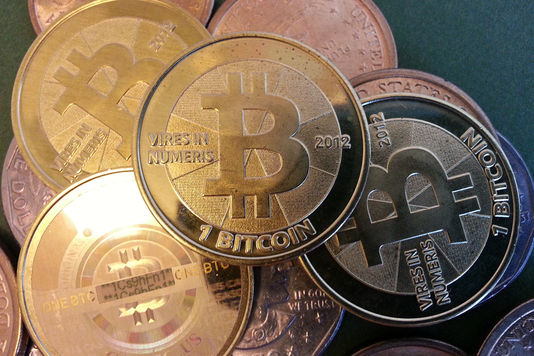
\includegraphics[width=10.00cm]{img/3156581_7_c614_le-systeme-de-monnaie-virtuelle-bitcoin_c7723fa59d263918a76b2f84261ccb14.jpg} ~\\
	\emph{Le syst{\`e}me de monnaie virtuelle bitcoin s'appuie sur un r{\'e}seau pair {\`a} pair pour {\'e}changer des unit{\'e}s de compte. | Flickr/Zach Copley}~\\
\end{minipage} \hfill \begin{minipage}[ht]{9.00cm}
	L'histoire de ses origines est aussi obscure et myst{\'e}rieuse que l'explication de son r{\'e}cent succ{\`e}s. Monnaie virtuelle au nom un peu barbare, longtemps apanage des seuls mordus de l'Internet, le "bitcoin" voit son cours litt{\'e}ralement flamber. ~\\
	
	\textbf{Lire notre article : " Bitcoin, les deux faces de la monnaie virtuelle"\footnotemark}~\\ 

	Mardi 9 avril au matin, la "e-devise" s'{\'e}changeait autour de 194 dollars (149 euros), alors qu'elle en valait moins de 20 en janvier. La valeur totale de bitcoins en circulation repr{\'e}sente quelque 2 milliards de dollars, soit un doublement en quelques jours. Une v{\'e}ritable fr{\'e}n{\'e}sie qui met sous les projecteurs cette monnaie largement inconnue du grand public. ~\\		
\end{minipage}~\\
\footnotetext{\texttt{http://www.lemonde.fr/technologies/article/2011/06/17/bitcoin-les-deux-faces-de-la-monnaie-virtuelle\_1537285\_651865.html}}

Le bitcoin est n{\'e} en janvier 2009. Son inventeur, un {\'e}nigmatique programmeur informatique dissimul{\'e} sous le pseudonyme Satoshi Nakamoto, semble poursuivre une ambition : la cr{\'e}ation d'une monnaie {\'e}chappant au contr{\^o}le des banques centrales et des Tr{\'e}sors nationaux. --- Celle-ci est mise au service d'un r{\'e}seau de transactions financi{\`e}res, d{\'e}centralis{\'e}, anonyme et sans frais visant {\`a} contourner le monopole des {\'e}tablissements bancaires. "\emph{Le bitcoin est bien plus qu'une simple devise}, d{\'e}crit Pierre Noizat, cofondateur de Paymium, une start-up sp{\'e}cialis{\'e}e dans le paiement en bitcoins. \emph{C'est aussi un r{\'e}seau et une technologie.}" ~\\

\textbf{11 MILLIONS DE BITCOINS EN CIRCULATION}~\\

Personne ne "poss{\`e}de" cette monnaie num{\'e}rique, {\'e}mise gr{\^a}ce {\`a} un puissant algorithme. Mais tous ceux qui consacrent la puissance de leur ordinateur {\`a} faire fonctionner le r{\'e}seau et {\`a} v{\'e}rifier l'authenticit{\'e} des transactions sont r{\'e}compens{\'e}s en bitcoins. Ils peuvent, ensuite, les revendre, sur Internet, sur une vingtaine de places de march{\'e}. Dont la plus importante, MtGox, est {\'e}tablie au Japon. ~\\

On recense autour de 11 millions de bitcoins en circulation. Le syst{\`e}me est programm{\'e} de telle sorte que le volume total, {\`a} terme, n'exc{\`e}de pas 21 millions. Aujourd'hui, les acteurs de l'{\'e}cosyst{\`e}me {\'e}valuent {\`a} quelques milliers le nombre de sites Web qui acceptent les bitcoins comme dons ou comme moyens de paiement. ~\\

Mais d'o{\`u} vient ce soudain acc{\`e}s de popularit{\'e} ? La crise chypriote est cit{\'e}e par des analystes : la crainte de voir leurs d{\'e}p{\^o}ts lourdement tax{\'e}s aurait pouss{\'e} de nombreux {\'e}pargnants {\`a} convertir leurs euros en bitcoins. "\emph{Mais il n'existe aucune preuve tangible, si ce n'est que les dates concordent}", nuance Yannick Naud de la soci{\'e}t{\'e} londonienne d'investissement Glendevon King Asset Management. ~\\

Pour ce g{\'e}rant, c'est d'abord la sp{\'e}culation qui est {\`a} l'oeuvre. Alors que le ph{\'e}nom{\`e}ne est aliment{\'e} par le brouhaha m{\'e}diatique et les r{\'e}seaux sociaux, "\emph{les gens ach{\`e}tent du bitcoin parce qu'ils pensent que sa valeur sera sup{\'e}rieure demain}", r{\'e}sume M. Naud. Lui-m{\^e}me re\c{c}oit de plus en plus de demandes d'information de clients depuis quelques jours. ~\\

\clearpage

\textbf{EXTR{\^E}ME VOLATILIT{\'E}}~\\

La fi{\`e}vre est telle que certains {\'e}voquent la formation d'une bulle sur le point de crever. D{\'e}j{\`a}, en 2011, le bitcoin {\'e}tait pass{\'e} de quelques centimes {\`a} 30 dollars avant de s'effondrer sous les 3 dollars en l'espace de cinq mois. "\emph{On n'est pas dans une bulle, on est dans une logique o{\`u} il faut mettre un prix sur quelque chose de nouveau}", d{\'e}fend M. Noizat qui souligne qu'apr{\`e}s quatre ans, le projet est sorti de sa phase purement exp{\'e}rimentale. ~\\

Mais, m{\^e}me ses promoteurs admettent que l'extr{\^e}me volatilit{\'e} du bitcoin nuit {\`a} son bon fonctionnement. "\emph{Les virements deviennent compliqu{\'e}s si la monnaie prend 10 euros en quelques heures}, note Philippe Herlin, {\'e}conomiste, charg{\'e} de cours au Conservatoire national des arts et m{\'e}tiers. \emph{Le bitcoin {\'e}tait dans l'enfance. Il entre dans l'adolescence avec son lot de crises.}" ~\\

En attendant, la devise se d{\'e}veloppe sous le regard attentif et suspicieux des autorit{\'e}s mon{\'e}taires. Dans un rapport d'octobre 2012, la Banque centrale europ{\'e}enne la d{\'e}crivait comme "\emph{la monnaie virtuelle ayant le plus de succ{\`e}s}". Tout en soulignant la n{\'e}cessit{\'e} de r{\'e}{\'e}valuer les risques si son usage venait {\`a} se g{\'e}n{\'e}raliser. ~\\

Aux Etats-Unis, les autorit{\'e}s se sont d{\'e}j{\`a} inqui{\'e}t{\'e}es de la libert{\'e} et de l'opacit{\'e} entourant le bitcoin. Le syst{\`e}me est suspect{\'e} d'{\^e}tre utilis{\'e} {\`a} des fins de blanchiment ou de trafic de drogue. ~\\

\emph{Marie de Verg{\`e}s --- Journaliste au Monde}~\\

\clearpage

\texttt{http://www.lemonde.fr/technologies/article/2013/04/12/chute-brutale-du-cours-de-la-monnaie-virtuelle-bitcoin\_3158844\_651865.html}~\\

\textbf{La chute brutale de bitcoin}~\\

\textbf{\small Le Monde.fr | 12.04.2013 {\`a} 17h33 --- Mis {\`a} jour le 12.04.2013 {\`a} 19h55}~\\

Apr{\`e}s avoir atteint des sommets, en d{\'e}but de semaine, la monnaie virtuelle bitcoin a connu, jeudi 11 avril, une chute brutale. S'inqui{\'e}tant d'une importante baisse du cours, mercredi, Mt. Gox, la principale plateforme de r{\'e}f{\'e}rence pour la conversion des bitcoins en dollars, {\`a} m{\^e}me d{\^u} en suspendre temporairement la cotation. ~\\

Le service a aussi connu une paralysie temporaire, mais Mt. Gox \texttt{se voulait rassurant\footnote{\texttt{https://mtgox.com/press\_release\_20130411.html}}}, jeudi. "\emph{Nous n'avons pas {\'e}t{\'e} victime d'une attaque de d{\'e}ni de service, mais nous avons plut{\^o}t {\'e}t{\'e} victime de notre succ{\`e}s}", explique un communiqu{\'e}. Selon Mt. Gox, les lenteurs de son site seraient en fait li{\'e}es {\`a} l'afflux de nouveaux utilisateurs. ~\\

Le bitcoin a {\'e}t{\'e} invent{\'e} en 2009 dans le sillage de la crise financi{\`e}re mondiale par Satoshi Nakamoto, pseudonyme d'un informaticien qui souhaitait cr{\'e}er une monnaie ne d{\'e}pendant d'aucune banque centrale ou institution financi{\`e}re. ~\\

\textbf{Lire : Le "bitcoin", une monnaie virtuelle qui s'arrache\footnote{\texttt{http://www.lemonde.fr/technologies/article/2013/04/09/le-bitcoin-une-monnaie-virtuelle-qu-on-s-arrache\_3156495\_651865.html}}} ~\\

Pour pouvoir {\'e}changer des bitcoins, les internautes doivent installer un logiciel sur leur ordinateur. Ces utilisateurs allouent d{\`e}s lors une partie de la capacit{\'e} de calcul de leur machine, et contribuent au processus de s{\'e}curisation des transactions. Ce syst{\`e}me permet {\'e}galement de g{\'e}n{\'e}rer, au compte-gouttes, de nouveaux bitcoins, un algorithme gratifiant au hasard un internaute pour sa contribution. Au total, Satoshi Nakamoto a pr{\'e}vu qu'environ 21 millions de bitcoins devraient {\^e}tre {\'e}mis d'ici {\`a} 2030, selon une courbe pr{\'e}visible. ~\\

Outre la "g{\'e}n{\'e}ration spontan{\'e}e" de cette monnaie virtuelle, une plateforme comme Mt. Gox permet de r{\'e}aliser des {\'e}changes contre des dollars ou des euros. C'est sur ce type de sites que les internautes peuvent constater l'ascension du bitcoin. En f{\'e}vrier, un bitcoin s'{\'e}changeait contre 20 dollars (15,3 euros). Le cours a brusquement augment{\'e} ces derni{\`e}res semaines, atteignant jusqu'{\`a} 237 dollars (182 euros), mercredi 10 avril, avant de rechuter brutalement, {\`a} 92 dollars vendredi (70 euros). Pour certains analystes, ces variations pourraient avoir {\'e}t{\'e} provoqu{\'e}es par des investisseurs russes et chypriotes cherchant {\`a} {\'e}viter la crise. ~\\

\textbf{Lire : Bitcoin, les deux faces de la monnaie virtuelle\footnote{\texttt{http://www.lemonde.fr/technologies/article/2011/06/17/bitcoin-les-deux-faces-de-la-monnaie-virtuelle\_1537285\_651865.html}}} ~\\

\textbf{DIVERSIFICATION DES INVESTISSEURS} ~\\

Par sa nature d{\'e}centralis{\'e}e et son syst{\`e}me de chiffrement, le bitcoin a d'abord suscit{\'e} l'inter{\^e}t des technophiles. Mais ces derniers mois, le bitcoin a peu {\`a} peu conquis un public plus large. A la fin de l'ann{\'e}e derni{\`e}re, la plateforme de blogs Wordpress a par exemple annonc{\'e} qu'elle accepterait le syst{\`e}me de monnaie bitcoin pour l'achat de certaines de ses fonctionnalit{\'e}s payantes. Certaines boutiques en ligne permettent aussi d'acheter des objets r{\'e}els... ~\\

Mais depuis sa m{\'e}diatisation, le \texttt{spectre d'une bulle\footnote{\texttt{http://arstechnica.com/business/2013/04/taming-the-bubble-investors-bet-on-bitcoin-via-derivatives-markets/}}} li{\'e}e au bitcoin est r{\'e}guli{\`e}rement agit{\'e}. Malgr{\'e} les variations de cours, les bitcoins semblent continuer {\`a} aiguiser les app{\'e}tits, y compris de nombreux investisseurs. ~\\

La presse am{\'e}ricaine rapporte que les fr{\`e}res Winklevoss, longtemps en guerre avec Mark Zuckerberg sur la propri{\'e}t{\'e} du r{\'e}seau social Facebook, \texttt{disposent d{\'e}sormais\footnote{\texttt{http://dealbook.nytimes.com/2013/04/11/as-big-investors-emerge-bitcoin-gets-ready-for-its-close-up/}}} de l'{\'e}quivalent de 11 millions de dollars (8,5 millions d'euros) de bitcoins. ~\\

\clearpage

\texttt{http://www.lemonde.fr/technologies/article/2013/08/12/une-faille-dans-android-permet-de-vider-les-porte-monnaies-virtuels-bitcoin\_3460383\_651865.html}~\\

\textbf{Les porte-monnaie Bitcoin compromis sur Android}~\\

\textbf{\small Le Monde.fr | 12.08.2013 {\`a} 12h58 --- Mis {\`a} jour le 12.08.2013 {\`a} 13h58}~\\

\begin{minipage}[ht]{10.25cm}
	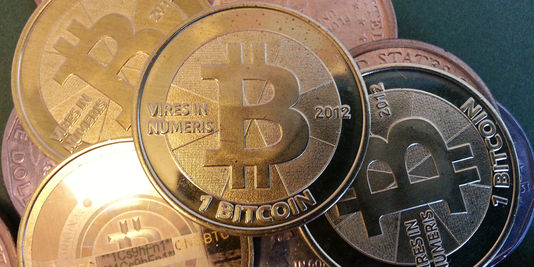
\includegraphics[width=10.00cm]{img/3156581_3_8f5d_le-systeme-de-monnaie-virtuelle-bitcoin_a85d434d2933b57b00d4d98f2c87cc10.jpg} ~\\
	\emph{ Le syst{\`e}me de monnaie virtuelle bitcoin s'appuie sur un r{\'e}seau pair {\`a} pair pour {\'e}changer des unit{\'e}s de compte. | Flickr/Zach Copley}~\\
\end{minipage} \hfill \begin{minipage}[ht]{9.00cm}
	Les d{\'e}veloppeurs de Bitcoin ont annonc{\'e} dans leur blog la d{\'e}couverte d'une faille critique dans Android qui permettrait {\`a} des personnes d'acc{\'e}der aux porte-monnaie virtuels des utilisateurs. Selon le site Generation-NT qui relaie l'information, lundi 12 ao{\^u}t, "\emph{la vuln{\'e}rabilit{\'e} touche actuellement toutes les applications de porte-monnaie Bitcoin sous Android, y compris les plus populaires comme Bitcoin Wallet, Blockchain.info wallet, BitcoinSpinner ou Mycelium Wallet}". ~\\	
\end{minipage}~\\

Les d{\'e}veloppeurs indiquent que la faille se situe dans la capacit{\'e} d'Android {\`a} g{\'e}n{\'e}rer des liens s{\'e}curis{\'e}s entre des chiffres al{\'e}atoires, ce qui est cens{\'e} s{\'e}curiser le stock de Bitcoin de l'utilisateur. Les services de change comme Mt Gox ou Coinbase ne sont pas concern{\'e}s par cette faille puisque leurs cl{\'e}s priv{\'e}es ne sont pas g{\'e}n{\'e}r{\'e}es depuis un dispositif Android. ~\\

"\emph{Il est actuellement conseill{\'e} aux utilisateurs ayant g{\'e}n{\'e}r{\'e} un porte-monnaie Bitcoin depuis une application Android de cr{\'e}er une nouvelle adresse {\`a} l'aide d'un g{\'e}n{\'e}rateur de cl{\'e} s{\'e}curis{\'e} dans le but de se renvoyer son propre stock de bitcoins}", poursuit le site. Des mises {\`a} jour des applications concern{\'e}es sont d{\'e}j{\`a} en d{\'e}veloppement. ~\\

\textbf{"BITCOIN N'EST PAS AUSSI S{\'E}CURIS{\'E} QUE CE QUE L'ON CROIT"} ~\\

Le bitcoin a {\'e}t{\'e} invent{\'e} en 2009 dans le sillage de la crise financi{\`e}re mondiale par un informaticien qui se cache derri{\`e}re le pseudonyme de Satoshi Nakamoto, qui souhaitait cr{\'e}er une monnaie ne d{\'e}pendant d'aucune banque centrale ou institution financi{\`e}re. ~\\

Une sorte d'"\emph{e-monnaie}" cr{\'e}{\'e}e {\`a} partir de morceaux de codes informatiques complexes g{\'e}n{\'e}r{\'e}s automatiquement par ordinateur, un processus appel{\'e} "frappe" et qui peu en th{\'e}orie {\^e}tre dupliqu{\'e} par n'importe quelle personne poss{\'e}dant un ordinateur. ~\\

"\emph{Bitcoin n'est pas aussi s{\'e}curis{\'e} que ce que l'on croit}", \texttt{avertissait ainsi en mars dernier Dan Kaminsky\footnote{\texttt{http://www.wired.com/opinion/2013/05/lets-cut-through-the-bitcoin-hype/}}}, sp{\'e}cialis{\'e} dans la s{\'e}curit{\'e} informatique. En juin 2011, des hackers s'en {\'e}taient d{\'e}j{\`a} pris {\`a} ces porte-monnaie virtuels qu'ils avaient vid{\'e}s {\`a} l'insu de leurs propri{\'e}taires. ~\\ 

\textbf{Lire : Le "bitcoin", une monnaie virtuelle qui s'arrache\footnote{\texttt{http://www.lemonde.fr/technologies/article/2013/04/09/le-bitcoin-une-monnaie-virtuelle-qu-on-s-arrache\_3156495\_651865.html}}} ~\\

\clearpage

\texttt{http://www.lemonde.fr/technologies/article/2013/08/20/berlin-reconnait-la-monnaie-virtuelle-bitcoin-pour-mieux-la-taxer\_3463593\_651865.html}~\\

\textbf{L'Allemagne reconna{\^i}t la monnaie virtuelle Bitcoin, pour mieux la taxer}~\\

\textbf{\small Le Monde.fr avec AFP | 20.08.2013 {\`a} 04h41 --- Mis {\`a} jour le 20.08.2013 {\`a} 07h34}~\\

%% \begin{minipage}[ht]{10.25cm}
	%% 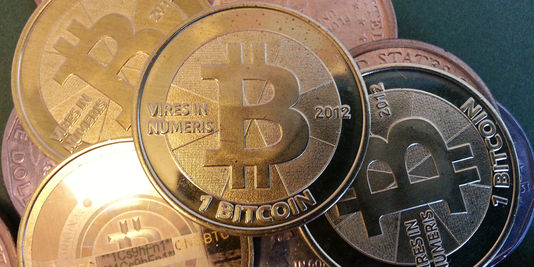
\includegraphics[width=10.00cm]{img/3156581_3_8f5d_le-systeme-de-monnaie-virtuelle-bitcoin_a85d434d2933b57b00d4d98f2c87cc10.jpg} ~\\
	%% \emph{ Le syst{\`e}me de monnaie virtuelle bitcoin s'appuie sur un r{\'e}seau pair {\`a} pair pour {\'e}changer des unit{\'e}s de compte. | Flickr/Zach Copley}~\\
%% \end{minipage} \hfill \begin{minipage}[ht]{9.00cm}
	Invent{\'e} en 2009 dans le sillage de la crise financi{\`e}re mondiale, le Bitcoin conquiert peu {\`a} peu une reconnaissance internationale. L'Allemagne a ainsi annonc{\'e} la reconnaissance officielle de la monnaie virtuelle comme "\emph{monnaie priv{\'e}e}", explique \texttt{lundi 19 ao{\^u}t le Huffington Post\footnotemark}. ~\\

	Gr{\^a}ce {\`a} ce statut juridique, tous les "\emph{{\'e}changes multilat{\'e}raux}" pourront {\^e}tre r{\'e}alis{\'e}s dans cette devise virtuelle en Allemagne. En contrepartie, Berlin ne cache pas son int{\'e}r{\^e}t dans l'op{\'e}ration : l'administration fiscale pourra en effet d{\'e}sormais pr{\'e}lever une taxe sur toutes ces transactions, qui {\'e}chappaient jusque-l{\`a} {\`a} l'imp{\^o}t. ~\\
%% \end{minipage}~\\
\footnotetext{\texttt{http://www.huffingtonpost.fr/2013/08/19/bitcoin-allemagne-monnaie-tva-taxe-hack-or\_n\_3779668.html?utm\_hp\_ref=tw}}

Et la part de Berlin est loin d'{\^e}tre n{\'e}gligeable, puisque les pr{\'e}l{\`e}vements se feront {\`a} hauteur de 25 \% sur les b{\'e}n{\'e}fices la premi{\`e}re ann{\'e}e. "\emph{Cela fonctionnera exactement comme la taxation sur les plus-values immobili{\`e}res. Concernant les entreprises, elles devront int{\'e}grer un taux de TVA dans toutes leurs transactions en bitcoins}", explique encore le Huffington Post. ~\\

\textbf{21 MILLIONS DE BITCOINS D'ICI {\`A} 2030} ~\\

Le Bitcoin a {\'e}t{\'e} lanc{\'e} par Satoshi Nakamoto, pseudonyme d'un informaticien qui souhaitait cr{\'e}er une monnaie ne d{\'e}pendant d'aucune banque centrale ou institution financi{\`e}re. Pour pouvoir {\'e}changer des bitcoins, les internautes doivent installer un logiciel sur leur ordinateur. Ces utilisateurs allouent d{\`e}s lors une partie de la capacit{\'e} de calcul de leur machine et contribuent au processus de s{\'e}curisation des transactions. Ce syst{\`e}me permet {\'e}galement de g{\'e}n{\'e}rer, au compte-gouttes, de nouveaux bitcoins, un algorithme gratifiant au hasard un internaute pour sa contribution. ~\\

\textbf{Lire nos explications : Bitcoin, BitTorrent, TOR : un Internet d{\'e}centralis{\'e} pour des usages centralis{\'e}s ?\footnote{\texttt{http://www.lemonde.fr/technologies/article/2013/08/14/un-internet-decentralise-pour-des-usages-centralises\_3460991\_651865.html}}} ~\\

Au total, Satoshi Nakamoto a pr{\'e}vu qu'environ 21 millions de bitcoins devraient {\^e}tre {\'e}mis d'ici {\`a} 2030, selon une courbe pr{\'e}visible. Outre la "\emph{g{\'e}n{\'e}ration spontan{\'e}e}" de cette monnaie virtuelle, une plateforme comme Mt. Gox permet de r{\'e}aliser des {\'e}changes contre des dollars ou des euros. En ao{\^u}t 2013, il s'{\'e}change ainsi pour environ 105 dollars, soit deux fois moins qu'au plus fort de la crise chypriote, o{\`u} il avait atteint un pic {\`a} 266 dollars. ~\\ 

\textbf{"LE FBI ET LA BCE CONSID{\`E}RENT LE PRODUIT COMME DOUTEUX"} ~\\

Par sa nature d{\'e}centralis{\'e}e et son syst{\`e}me de chiffrement, le bitcoin a d'abord suscit{\'e} l'inter{\^e}t des technophiles. Mais ces derni{\`e}res ann{\'e}es le bitcoin a peu {\`a} peu conquis un public plus large. La plateforme de blogs Wordpress a ainsi annonc{\'e} qu'elle accepterait le syst{\`e}me de monnaie Bitcoin pour l'achat de certaines de ses fonctionnalit{\'e}s payantes. Certaines boutiques en ligne permettent aussi d'acheter des objets r{\'e}els... ~\\

Mais depuis sa m{\'e}diatisation, le spectre d'une bulle li{\'e}e au bitcoin est r{\'e}guli{\`e}rement agit{\'e}. Malgr{\'e} les variations de cours, les bitcoins semblent continuer {\`a} aiguiser les app{\'e}tits, y compris de nombreux investisseurs. D'autres pays se sont {\'e}galement r{\'e}cemment montr{\'e}s int{\'e}ress{\'e}s par une reconnaissance du bitcoin, notamment l'Australie et les Etats-Unis. --- "\emph{A contrario, le FBI et la BCE consid{\`e}rent le produit comme douteux, tandis que la Tha{\"i}lande a carr{\'e}ment banni son utilisation}", explique le Huff Post. Il existe en effet des failles de s{\'e}curit{\'e} qui pr{\'e}sentent un risque non n{\'e}gligeable pour les utilisateurs de la monnaie virtuelle. Les porte-monnaies h{\'e}berg{\'e}s sur Android ont par exemple subi des attaques r{\'e}cemment, rappelle le site d'information. ~\\

\clearpage

\texttt{http://abonnes.lemonde.fr/economie/article/2013/09/20/le-bitcoin-monnaie-trublion\_3481598\_3234.html}~\\

\textbf{Le bitcoin, monnaie trublion}~\\

\textbf{\small LE MONDE | 20.09.2013 {\`a} 11h43 --- Mis {\`a} jour le 20.09.2013 {\`a} 14h26 | Par Marie Charrel  }~\\

\begin{minipage}[ht]{10.25cm}
	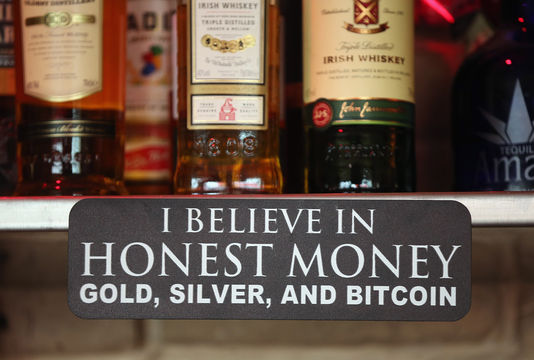
\includegraphics[width=10.00cm]{img/3481688_6_af19_au-room-77-dans-le-quartier-kreuzberg-a_817c1632a0fcd91dda95a5df6039a5ed.jpg} ~\\
	\emph{Au Room 77, dans le quartier Kreuzberg, {\`a} Berlin, les clients peuvent r{\'e}gler leurs consommations avec des bitcoins.| Sean Gallup/Getty Images/AFP}~\\
\end{minipage} \hfill \begin{minipage}[ht]{9.00cm}
	Ne lui parlez plus d'euros. Joerg Platzer, lui, ne jure que par le bitcoin. Au Room 77, le bar qu'il poss{\`e}de {\`a} Kreuzberg, dans la capitale allemande, les clients peuvent commander une bi{\`e}re et des burritos et payer avec cette myst{\'e}rieuse monnaie {\'e}lectronique. "\emph{C'est plus rapide qu'un paiement par carte bancaire, explique-t-il. Il leur suffit d'un clic sur l'application iPhone d{\'e}di{\'e}e.}" ~\\
	
	Dans son quartier, fer de lance de la culture branch{\'e}e berlinoise, une quarantaine de commer\c{c}ants se sont, comme lui, convertis aux bitcoins. "\emph{Si \c{c}a continue, on pourra bient{\^o}t se passer des billets {\`a} l'ancienne}", se r{\'e}jouit Thomas, jeune cadre habitant le coin. Lui et Joerg Platzer en sont convaincus : le bitcoin est sur le point de changer le monde. ~\\
\end{minipage}~\\

Des doux dingues ? Peut-{\^e}tre. Mais ils ne sont pas les seuls. Partout dans le monde, des milliers de commerces en ligne comme traditionnels s'y sont mis, de la c{\'e}l{\`e}bre plate-forme de blogs WordPress {\`a} des loueurs de voitures am{\'e}ricains en passant par des maisons d'h{\^o}tes en Toscane. Chez nous, des dizaines d'e-boutiques (Cosmevert. com, Electrocig-boutique. fr, Miniplanes. fr...) et m{\^e}me certaines annonces sur Leboncoin.fr acceptent la devise. ~\\

Si bien que les grands r{\'e}gulateurs financiers commencent {\`a} s'y int{\'e}resser car, pour l'instant, le bitcoin, sans {\^e}tre ill{\'e}gal, ne rentre dans aucune cat{\'e}gorie juridique pr{\'e}cise. En ao{\^u}t, \texttt{l'Allemagne lui a donn{\'e} le statut officiel de "monnaie priv{\'e}e"\footnote{\texttt{http://www.lemonde.fr/technologies/article/2013/08/20/berlin-reconnait-la-monnaie-virtuelle-bitcoin-pour-mieux-la-taxer\_3463593\_651865.html}}}, ce qui lui permettra de taxer 25 \% des b{\'e}n{\'e}fices g{\'e}n{\'e}r{\'e}s. ~\\

\textbf{"NORMALISATION"} ~\\

De son c{\^o}t{\'e}, le S{\'e}nat am{\'e}ricain consulte en ce moment les acteurs du milieu afin de plancher sur une r{\'e}gulation adapt{\'e}e. Le 14 septembre, le gouvernement britannique a, dans le m{\^e}me but, re\c{c}u des start-up utilisant la devise num{\'e}rique. L'Australie, le Canada, la Belgique et les Pays-Bas songent {\`a} faire de m{\^e}me... "\emph{L'utilisation du bitcoin est en train de se normaliser}", s'enthousiasme Gonzague Grandval, le patron de Paymium, une start-up fran\c{c}aise sur le cr{\'e}neau. ~\\

Dr{\^o}le de destin pour cette {\'e}trange monnaie {\`a} la r{\'e}putation sulfureuse. Son histoire semble tout droit sortie d'un roman de Philip K. Dick. Elle aurait {\'e}t{\'e} cr{\'e}{\'e}e en 2009 par un ou plusieurs informaticiens se pr{\'e}sentant sous le pseudonyme de Satoshi Nakamoto. L'objectif : cr{\'e}er une devise {\'e}chappant au contr{\^o}le des Etats et, donc, non soumise {\`a} la tentation de la "planche {\`a} billets", un mal selon eux {\`a} l'origine de crises telles que celle des subprimes. ~\\

Jusqu'en 2012, l'invention ne d{\'e}passa pas le cercle des f{\'e}rus de cryptographie et de codage num{\'e}rique. Il faut dire que son fonctionnement d{\'e}fie la compr{\'e}hension du commun des mortels. --- Les bitcoins {\'e}chappent {\`a} toutes les r{\`e}gles mon{\'e}taires classiques. Ils ne sont pas cr{\'e}{\'e}s par le cycle des pr{\^e}ts bancaires, comme les euros ou les dollars, et ne sont pas contr{\^o}l{\'e}s par une banque centrale. ~\\

\clearpage

\textbf{UN ALGORITHME INFORMATIQUE} ~\\

Leur {\'e}mission est g{\'e}r{\'e}e par un algorithme informatique, programm{\'e} pour g{\'e}n{\'e}rer r{\'e}guli{\`e}rement et {\`a} un rythme d{\'e}croissant des bitcoins. Et ce, jusqu'{\`a} ce que leur montant, aujourd'hui de 11 millions, atteigne 21 millions, aux alentours de 2035. "\emph{C'est un peu comme une mati{\`e}re premi{\`e}re telle que l'or : la source se tarira un jour, et c'est en partie de l{\`a} que le bitcoin tire sa valeur}", explique M. Platzer. ~\\

Concr{\`e}tement, l'algorithme fonctionne gr{\^a}ce {\`a} des passionn{\'e}s d'informatique, devenus des quasi-professionnels du genre. Surnomm{\'e}s "mineurs", ils mettent en commun leurs ordinateurs au service du r{\'e}seau. Chaque fois qu'ils r{\'e}solvent un certain nombre d'{\'e}quations, ces mineurs re\c{c}oivent un petit montant de bitcoins en r{\'e}compense, qu'ils revendent ou d{\'e}pensent {\`a} leur gr{\'e}. ~\\

Mais quelle est l'utilit{\'e} de cette cha{\^i}ne de calcul, au juste ? C'est l{\`a} toute la complexit{\'e} et l'int{\'e}r{\^e}t de la technologie : elle sert {\`a} valider et r{\'e}pertorier les transactions effectu{\'e}es partout dans le monde en bitcoins. Une base de donn{\'e}es publique, {\`a} laquelle tout le monde peut avoir acc{\`e}s. Et qui {\'e}vite que des petits malins ne cr{\'e}ent de faux bitcoins : ces derniers seraient rejet{\'e}s par le r{\'e}seau. "\emph{Le bitcoin est donc {\`a} la fois une monnaie et un protocole de paiement}", r{\'e}sume Philippe Herlin, {\'e}conomiste au Conservatoire national des arts et des m{\'e}tiers. Plut{\^o}t obscur... ~\\

C{\^o}t{\'e} utilisateurs, les choses sont un peu plus simples. Ces derniers peuvent acheter des bitcoins en se rendant sur l'une des places de march{\'e} en ligne, comme MtGox, Bitstamp ou Bitcoin-Central. Leurs bitcoins sont alors stock{\'e}s sur un portefeuille num{\'e}rique h{\'e}berg{\'e} sur leur ordinateur, smartphone ou sur un site Web d{\'e}di{\'e}. ~\\

\textbf{LIMITER LES RISQUES DE BLANCHIMENT} ~\\

Des ventes sont {\'e}galement organis{\'e}es tous les mois dans quelques grandes villes, comme au "Satoshi Square", dans le quartier new-yorkais d'Union Square. Comme sur un march{\'e} classique, les aficionados s'y {\'e}changent des bitcoins, gr{\^a}ce {\`a} leur mobile. Enfin, plusieurs compagnies sp{\'e}cialis{\'e}es commencent {\`a} installer aux quatre coins du monde des distributeurs automatiques : l{\`a} aussi, les bitcoins sont retir{\'e}s par l'interm{\'e}diaire du mobile ou de cartes pr{\'e}pay{\'e}es. ~\\

Dans tous les cas, si les transactions sont publiques, l'identit{\'e} des utilisateurs, elle, reste crypt{\'e}e. Un anonymat qui n'a bien s{\^u}r pas tard{\'e} {\`a} attirer trafics et blanchiment en tout genre. En 2011, Silk Road, un site ill{\'e}gal de vente de drogue, fit du bitcoin sa monnaie de pr{\'e}dilection. ~\\

Les sites utilisant la devise sont r{\'e}guli{\`e}rement attaqu{\'e}s par des hackers, et des sp{\'e}culateurs profitent de la forte volatilit{\'e} de la devise pour engranger des profits. "\emph{Ce sont des maux de jeunesse qui seront bient{\^o}t derri{\`e}re nous}", assure Gonzague Gay-Bouchery, patron de MtGox, la plus grosse place d'{\'e}change de la devise. ~\\

\textbf{Lire : Les porte-monnaie Bitcoin compromis sur Android\footnote{\texttt{http://abonnes.lemonde.fr/technologies/article/2013/08/12/une-faille-dans-android-permet-de-vider-les-porte-monnaies-virtuels-bitcoin\_3460383\_651865.html}}} ~\\

De fait, les plates-formes comme la sienne, d{\'e}sireuses de t{\'e}moigner leur bonne volont{\'e} aux r{\'e}gulateurs, exigent d{\'e}sormais des utilisateurs de fournir une pi{\`e}ce d'identit{\'e} et un justificatif de domicile, afin de limiter les risques de blanchiment. ~\\

\textbf{COMME DU CASH NUM{\'E}RIQUE} ~\\

Reste une question-cl{\'e} : pourquoi cette monnaie suscite-t-elle un tel engouement ? Pour certains observateurs, il est surtout li{\'e} {\`a} la crise et {\`a} la m{\'e}fiance envers le syst{\`e}me bancaire qui s'ensuit. Au plus fort de la crise chypriote, des {\'e}pargnants ont ainsi utilis{\'e} le bitcoin pour contourner la limitation de sortie de capitaux, faisant s'envoler le cours du bitcoin au-del{\`a} de 260 dollars (192 euros), avant qu'il ne retombe {\`a} 80 dollars, puis s'{\'e}tablisse {\`a} 139 dollars. ~\\

\textbf{Lire : Chute brutale du cours de la monnaie virtuelle bitcoin\footnote{\texttt{http://abonnes.lemonde.fr/technologies/article/2013/04/12/chute-brutale-du-cours-de-la-monnaie-virtuelle-bitcoin\_3158844\_651865.html}}} ~\\

Une volatilit{\'e} affolante, faisant dire {\`a} de nombreux experts que la devise de Satoshi Nakamoto restera un {\'e}piph{\'e}nom{\`e}ne sp{\'e}culatif. "\emph{Elle n'a aucune utilit{\'e} {\'e}conomique et est vou{\'e}e {\`a} s'autod{\'e}truire}", pr{\'e}dit Yannick Naud, de la soci{\'e}t{\'e} d'investissement Glendevon King AM. ~\\

D'autres sont moins cat{\'e}goriques. Et soulignent que l'int{\'e}r{\^e}t de la monnaie num{\'e}rique tient surtout {\`a} la r{\'e}volution qu'elle repr{\'e}sente en termes de mode de paiement. "\emph{Elle est au virement bancaire classique ce que l'e-mail est au courrier papier}", r{\'e}sume Christian Parisot, {\'e}conomiste chez Aurel BCG. ~\\

Le bitcoin fonctionne en effet comme du cash num{\'e}rique : il passe d'un e-portefeuille {\`a} l'autre en quelques minutes -- et non apr{\`e}s un d{\'e}lai de vingt-quatre ou quarante-huit heures --, et de fa\c{c}on irr{\'e}versible. Surtout, il est assorti de frais de transaction quasi nuls, contrairement aux virements classiques et par carte bancaire, o{\`u} Master Card, Visa, PayPal ou Western Union pr{\'e}l{\`e}vent des commissions de 1,5 \% {\`a} 7 \% selon les pays. La pseudo-devise ne sert alors que d'interm{\'e}diaire. ~\\

\textbf{PAIEMENT QUASI INSTANTAN{\'E} ET LIBRE DE FRAIS BANCAIRES} ~\\

Prenons le cas d'un internaute souhaitant acheter une cl{\'e} USB sur le site de mat{\'e}riel {\'e}lectronique fran\c{c}ais Achatnet.pro. Lorsqu'il valide sa commande, une plate-forme sp{\'e}cialis{\'e}e nomm{\'e} BitPay convertit ses euros en bitcoins, cr{\'e}dite le compte du commer\c{c}ant, puis les convertis {\`a} nouveau en euros. Pour ce, BitPay a pr{\'e}lev{\'e} une commission de 0,99 \% seulement. "\emph{C'est une belle {\'e}conomie}", explique Patrick Ferrer, le patron d'Achatnet.pro. Bon joueur, il en fait profiter ses clients en leur offrant une ristourne de 3 \%. ~\\

Un paiement quasi instantan{\'e} et libre de frais bancaires : conscientes du potentiel commercial de ce syst{\`e}me, des dizaines de start-up se lancent sur le cr{\'e}neau en Europe et surtout aux Etats-Unis, o{\`u} elles attirent d{\'e}j{\`a} les convoitises des business angels : Paymium, Coinsetter, Cointbase, Bitinstant... ~\\

Des grands acteurs du Web, comme les fondateurs d'Ebay et Google, ont {\'e}galement confi{\'e} s'y int{\'e}resser de pr{\`e}s. "\emph{Cette technologie est susceptible d'{\'e}branler le monopole des acteurs bancaires sur les modes de paiement}", r{\'e}sume Philippe Herlin. "\emph{Quand il sera r{\'e}gul{\'e}, le bitcoin offrira des co{\^u}ts bien moins attractifs}", r{\'e}torque Yannick Naud. ~\\

Peut-{\^e}tre. Reste que, m{\^e}me si le bitcoin s'effondrait, il est loin d'{\^e}tre la seule innovation dans les tuyaux. Outre les autres monnaies {\'e}lectroniques fleurissant depuis quelques mois (ripple, litecoin, solidcoin...), l'Amazon Coin ou encore le paiement par SMS d{\'e}velopp{\'e} par Orange en Afrique (Orange Money) pr{\'e}sentent tous une alternative au virement bancaire classique. ~\\

\textbf{Lire : Avec Amazon Coin, le distributeur s'{\'e}loigne des banques\footnote{\texttt{http://abonnes.lemonde.fr/economie/article/2013/09/20/avec-amazon-coin-le-distributeur-s-eloigne-des-banques\_3481600\_3234.html}}}~\\

\emph{Marie Charrel}~\\


\clearpage

\texttt{http://www.lemonde.fr/technologies/article/2013/10/03/silk-road-ferme-et-alors\_3488971\_651865.html}~\\

\textbf{Silk Road ferme, et alors ?}~\\

\textbf{\small Le Monde.fr | 03.10.2013 {\`a} 13h08 --- Mis {\`a} jour le 03.10.2013 {\`a} 14h57 | Par \textbf{Charlotte Chabas} }~\\

\begin{minipage}[ht]{10.25cm}
	
\includegraphics[width=10.00cm]{img/3489421_3_e9f5_capture-ecran-du-site-silk-road_a5297453ba95c8e1e96a3d54fce55dd5.jpg} ~\\
	\emph{Capture {\'e}cran du site Silk Road. | D.R.}~\\
\end{minipage} \hfill \begin{minipage}[ht]{9.00cm}
	\textbf{Silk Road, qu'est-ce que c'{\'e}tait ?}~\\

	"Super qualit{\'e} pour de l'h{\'e}ro{\"i}ne qui d{\'e}fonce". \texttt{Voil{\`a} le type d'annonce\footnotemark} que l'on pouvait trouver sur Silk Road ("route de la soie"), jusqu'au mercredi 2 octobre, \texttt{date {\`a} laquelle la justice am{\'e}ricaine a annonc{\'e} avoir ferm{\'e} le site Internet\footnotemark }. Selon les autorit{\'e}s am{\'e}ricaines, le site {\'e}tait "\emph{un vaste march{\'e} noir en ligne o{\`u} {\'e}taient r{\'e}guli{\`e}rement achet{\'e}s et vendus des centaines de kilos de drogue et d'autres produits et services illicites}". ~\\
\end{minipage}~\\
\footnotetext{\texttt{http://www.rollingstone.com/culture/news/fbi-shuts-down-silk-road-20131002}}
\footnotetext{\texttt{http://www.lemonde.fr/technologies/article/2013/10/02/drogues-le-proprietaire-du-site-silk-road-arrete\_3488797\_651865.html}}

Concr{\`e}tement, Silk Road reposait sur un grand principe : l'anonymat. Le site, dissimul{\'e} dans le "deep web", c'est-{\`a}-dire cette partie du web non index{\'e}e par les moteurs de recherche classiques, n'{\'e}tait accessible qu'aux utilisateurs du r{\'e}seau d{\'e}centralis{\'e} TOR, qui garantit un anonymat complet. Lanc{\'e} en 2011, Silk Road permettait donc {\`a} ses utilisateurs de vendre ou d'acheter n'importe quel produit, et notamment de la drogue. Les cartes de cr{\'e}dit et les comptes Paypal {\'e}taient {\'e}videmment interdits, pour garantir la s{\'e}curit{\'e} des identit{\'e}s des utilisateurs. Pour r{\'e}gler les achats, les internautes utilisaient en effet la monnaie virtuelle "bitcoin", qui garantit la confidentialit{\'e} : les transactions y sont anonymes, et le vendeur ne conna{\^i}t pas l'acheteur. La seule information r{\'e}v{\'e}l{\'e}e {\'e}tait l'adresse de livraison. ~\\

\textbf{Lire (en {\'e}dition abonn{\'e}s) : "Le bitcoin, monnaie trublion"\footnote{\texttt{http://www.lemonde.fr/economie/article/2013/09/20/le-bitcoin-monnaie-trublion\_3481598\_3234.html}}} ~\\

Du cannabis {\`a} l'ecstasy, en passant par le LSD ou la coca{\"i}ne, "\emph{plusieurs milliers de dealers}" postaient ainsi leur annonce, et laissaient les acheteurs s{\'e}lectionner leur produit. \texttt{On trouvait {\'e}galement sur le site\footnote{\texttt{http://www.baltimoresun.com/news/maryland/crime/blog/bs-md-silk-road-shut-down-20131002,0,7548092.story?page=1}}} des manuels pour hacker des distributeurs d'argent, des armes, ou encore des contacts de faux-monnayeurs. Le site \texttt{avait toutefois pos{\'e} certaines restrictions\footnote{\texttt{http://www.wired.com/threatlevel/2013/10/silk-road-raided/}}} : la vente d'armes de destruction massive, de donn{\'e}es de cartes bancaires vol{\'e}es, ou encore la proposition de service pour assassiner des gens {\'e}taient ainsi interdits par le r{\`e}glement int{\'e}rieur du site. --- Selon le FBI, entre f{\'e}vrier 2011 et juillet 2013, le site a permis pr{\`e}s de 1,2 million de transactions, pour un montant total de pr{\`e}s de 9,5 millions de bitcoins, soit, selon les calculs des autorit{\'e}s am{\'e}ricaines, pr{\`e}s de 1,2 milliard de dollars. Silk Road pr{\'e}levait une commission sur chaque paiement, {\'e}valu{\'e}e sur la m{\^e}me p{\'e}riode {\`a} 600 000 bitcoins, soit 80 millions de dollars. Une somme qui permettait de financer le fonctionnement du site et la petite {\'e}quipe qui le g{\'e}rait. ~\\

	\textbf{Comment le FBI a men{\'e} cette op{\'e}ration ?}~\\

Plusieurs volets de l'enqu{\^e}te ont men{\'e} {\`a} la fermeture du site, mercredi, et {\`a} l'arrestation de son fondateur, Ross William Ulbricht. En juillet, \texttt{le FBI a r{\'e}ussi {\`a} identifier un serveur\footnote{\texttt{http://www.wired.com/threatlevel/2013/10/silk-road-raided/}}} situ{\'e} {\`a} l'{\'e}tranger, qui h{\'e}bergeait Silk Road. Gr{\^a}ce {\`a} une coop{\'e}ration avec les autorit{\'e}s locales, les enqu{\^e}teurs am{\'e}ricains ont pu obtenir une image claire du serveur, et acc{\'e}der aux messages priv{\'e}s {\'e}chang{\'e}s sur le site. ~\\

\clearpage

Pour parvenir ensuite {\`a} identifier les cr{\'e}ateurs de Silk Road, le FBI et les autres agences de s{\'e}curit{\'e} am{\'e}ricaines ont cherch{\'e} les premi{\`e}res traces en ligne de promotion du site, notamment sur les forums. C'est par ce biais que les enqu{\^e}teurs ont trouv{\'e} deux messages d'un certain "Altoid", qui leur a permis ensuite, par des recoupements, de trouver la trace d'un blog h{\'e}berg{\'e} par Wordpress, li{\'e} {\`a} une adresse Gmail. Il s'agissait de celle de Ross William Ulbricht, le fondateur du site. ~\\

	\textbf{Qui est le fondateur du site ?}~\\

Ross William Ulbricht, 29 ans, {\'e}tait connu sur Silk Road sous le pseudonyme de "Dread Pirate Roberts", ou "DPR", en r{\'e}f{\'e}rence {\`a} un personnage du livre \emph{Princess Bride}, le terrible pirate Roberts, connu pour son masque noir et sa propension {\`a} ne jamais faire de prisonniers. Selon les informations du FBI, Ulbricht {\'e}tait install{\'e} {\`a} San Francisco. Dipl{\^o}m{\'e} d'un master en science des mat{\'e}riaux {\`a} l'universit{\'e} de Pennsylvanie, le jeune homme contr{\^o}lait les serveurs et les infrastructures du site, {\'e}tait {\`a} l'origine du r{\`e}glement interne au site, g{\'e}rait un "service apr{\`e}s-vente" r{\'e}duit, et dirigeait une petite {\'e}quipe d'administrateurs. ~\\ 

\begin{minipage}[ht]{10.25cm}
	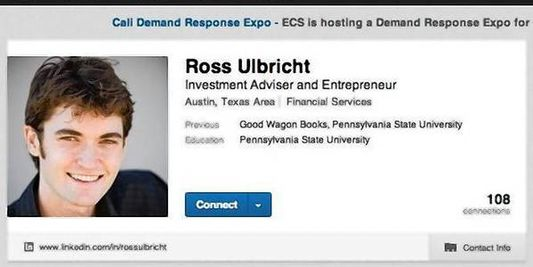
\includegraphics[width=10.00cm]{img/3489419_3_624f_profil-linkedin-de-ross-william-ulbricht_5e9a51b897c9680fb84211c1d0cc98b9.jpg} ~\\
	\emph{Profil LinkedIn de Ross William Ulbricht. | LinkedIn}~\\
\end{minipage} \hfill \begin{minipage}[ht]{9.00cm}
	Sur son profil Google +, Ross William Ulbricht se d{\'e}crivait comme un "libertarien {\'e}conomique et philosophique", et postait des vid{\'e}os de l'institut Ludwig von Mises, une organisation universitaire libertarienne d{\'e}di{\'e}e {\`a} l'enseignement et la recherche en philosophie et {\'e}conomie politique. ~\\ 

	\texttt{Interview{\'e} par \emph{Forbes} en ao{\^u}t 2013\footnotemark }, il expliquait que son site {\'e}tait, selon lui, "\emph{une exp{\'e}rience libertarienne qui ne fait pas de victime}". ~\\
\end{minipage} ~\\
\footnotetext{\texttt{http://www.forbes.com/sites/andygreenberg/2013/08/14/an-interview-with-a-digital-drug-lord-the-silk-roads-dread-pirate-roberts-qa/}}

	\textbf{Que lui reproche-t-on ?}~\\

Ross William Ulbricht a {\'e}t{\'e} inculp{\'e} mercredi pour trafic de drogue, blanchiment d'argent et piratage informatique. Mais le fondateur de Silk Road est {\'e}galement accus{\'e} de tentatives de meurtres. ~\\

\texttt{Selon le \emph{Baltimore Sun}\footnote{\texttt{http://www.baltimoresun.com/news/maryland/crime/blog/bs-md-silk-road-shut-down-20131002,0,7548092.story?page=1}}}, le FBI enqu{\^e}te en effet sur deux cas suspects dans lesquels Ross William Ulbricht a jou{\'e} un r{\^o}le de premier plan. En avril 2012, le fondateur de Silk Road est en effet accus{\'e} d'avoir demand{\'e} {\`a} un contact d'abattre l'un de ses employ{\'e}s, qu'il soup\c{c}onnait de vouloir r{\'e}v{\'e}ler son identit{\'e} et celui de plusieurs personnes li{\'e}es au site. Le "contact" {\'e}voqu{\'e} par les enqu{\^e}teurs {\'e}tait en r{\'e}alit{\'e} un agent du FBI infiltr{\'e}, qui a fait croire {\`a} Ulbricht que le meurtre avait bien eu lieu, envoyant notamment des photos de l'employ{\'e} en question tortur{\'e}. Le 1er mars 2012, Ross William Ulbricht envoyait 80 000 dollars, provenant d'un compte bancaire australien, vers le compte bancaire contr{\^o}l{\'e} par le FBI. "\emph{Je n'avais jamais tu{\'e} ou fait tuer quelqu'un avant, mais c'{\'e}tait ce qu'il fallait faire dans ce cas}", explique-t-il dans un message {\`a} son "contact". ~\\

En mars, des messages priv{\'e}s analys{\'e}s par le FBI montrent une deuxi{\`e}me affaire similaire. Ross William Ulbricht {\'e}crit ainsi qu'il veut "\emph{mettre un prix sur sa t{\^e}te}", en parlant d'un utilisateur du site, connu sous le pseudonyme "FriendlyChemist", qui avait menac{\'e} de divulguer des informations sur un autre utilisateur, "Redandwhite", qui lui devait de l'argent. "\emph{Des besoins comme \c{c}a, \c{c}a arrive de temps en temps pour une personne avec des responsabilit{\'e}s comme moi}", justifie-t-il dans ses messages, n{\'e}gociant m{\^e}me le prix du "service". Selon le \emph{Baltimore Sun}, on ignore encore ce qu'il est advenu de "FriendlyChemist", car aucune trace d'un tel meurtre n'appara{\^i}t dans les registres policiers. ~\\

\clearpage

	\textbf{Quelles sont les cons{\'e}quences de cette fermeture ?}~\\

La fermeture de Silk Road a imm{\'e}diatement provoqu{\'e} une vague de r{\'e}actions \texttt{sur le site de discussion Reddit\footnote{\texttt{http://www.reddit.com/r/SilkRoad/}}}. De nombreux utilisateurs se plaignent d'avoir perdu leur argent, {\`a} l'image de "IllJackYouOffSoHard", qui a envoy{\'e} 400 dollars quelques secondes avant que le site soit ferm{\'e}. "\emph{Je ne peux m{\^e}me pas imaginer combien d'argent les gens ont perdu aujourd'hui}", se lamente aussi "Luckyskyhigher". ~\\

\begin{minipage}[ht]{10.25cm}
	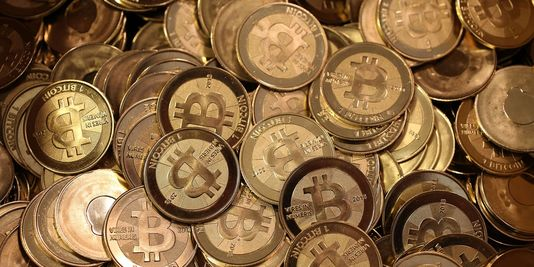
\includegraphics[width=10.00cm]{img/3489417_3_e452_de-la-monnaie-bitcoin-utilisee-notamment-par_c1731595dcf6cff3fe3dabaec5cd41f8.jpg} ~\\
	\emph{De la monnaie bitcoin, utilis{\'e}e notamment par le site Silk Road pour ses transactions entre utilisateurs. | AFP/GEORGE FREY}~\\
\end{minipage} \hfill \begin{minipage}[ht]{9.00cm}
	Plus grave, la fermeture du site pourrait avoir un impact cons{\'e}quent sur le march{\'e} du bitcoin. \texttt{Selon des experts cit{\'e}s par le \emph{New York Times}\footnotemark}, Silk Road concentrait pr{\`e}s de la moiti{\'e} des transactions r{\'e}alis{\'e}es en bitcoins. Depuis mercredi, le FBI a d'ailleurs saisi plus de 26 000 bitcoins, soit 3,6 millions de dollars, d{\'e}tenus par le site Internet. Le cours de la monnaie virtuelle a d'ailleurs fortement chut{\'e} apr{\`e}s l'annonce du FBI, perdant jusqu'{\`a} 20 \% de sa valeur : ~\\
\end{minipage} ~\\
\footnotetext{\texttt{http://www.nytimes.com/2013/10/03/nyregion/operator-of-online-market-for-illegal-drugs-is-charged-fbi-says.html?\_r=1\&}}

\begin{minipage}[ht]{9.00cm}
	\texttt{Mais le constat n'est pas si alarmant, selon Bloomberg\footnotemark }, qui affirme que "\emph{bitcoin n'a plus besoin aujourd'hui de Silk Road}". "\emph{La monnaie pr{\'e}sente toujours des risques importants, mais le fait qu'elle ait {\`a} l'avenir une base de clients faite de start-ups l{\'e}gales plut{\^o}t que de barons de la drogue ne peut {\^e}tre qu'une bonne chose pour son d{\'e}veloppement}", conclut l'agence de presse {\'e}conomique. La fin de la moiti{\'e} de l'activit{\'e} de bitcoin pourrait, {\`a} terme, donner une meilleure r{\'e}putation {\`a} cette monnaie virtuelle souvent accus{\'e}e de couvrir des activit{\'e}s ill{\'e}gales. ~\\
\end{minipage} \hfill \begin{minipage}[ht]{10.25cm}
	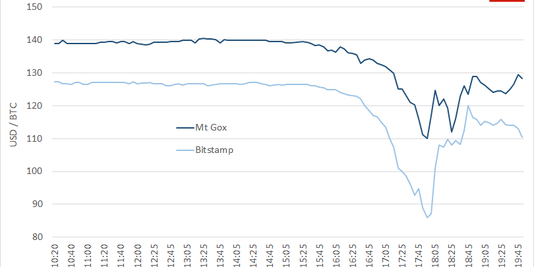
\includegraphics[width=10.00cm]{img/3489413_3_02cf_cours-du-bitcoin-mercredi-2-octobre_f0f554e8ec06f798d5e2d9f90f9c56d1.png} ~\\
	\emph{Cours du bitcoin, mercredi 2 octobre.}~\\
\end{minipage} ~\\
\footnotetext{\texttt{http://www.bloomberg.com/news/2013-10-02/will-silk-road-bust-kill-bitcoin-.html}}

\textbf{Lire : "Bitcoin, les deux faces de la monnaie virtuelle"~\footnote{\texttt{http://www.lemonde.fr/technologies/article/2011/06/17/bitcoin-les-deux-faces-de-la-monnaie-virtuelle\_1537285\_651865.html}} }~\\

Enfin, pour les anciens clients de Silk Road, le bilan n'est pas plus sombre. \texttt{Comme le rappelle Business Insider\footnote{\texttt{http://www.businessinsider.com/silk-road-alternatives-2013-10}}}, il existe toujours des alternatives. ~\\

\emph{Charlotte Chabas --- Journaliste au Monde}~\\ 

\clearpage

\texttt{http://www.numerama.com/magazine/20727-hadopi-couper-les-flux-financiers-du-piratage-peut-il-vraiment-fonctionner-maj.html}~\\

\textbf{Hadopi : couper les flux financiers du piratage peut-il vraiment fonctionner ? (M{\`a}J)}~\\

\emph{\small  Guillaume Champeau -- publi{\'e} le Mardi 13 D{\'e}cembre 2011 {\`a} 10h20 -- post{\'e} dans Soci{\'e}t{\'e} 2.0 }~\\

\textbf{L'Hadopi veut s'attaquer aux flux financiers pour lutter contre les plateformes de streaming et de t{\'e}l{\'e}chargement direct. Mais cette m{\'e}thode risque d'{\^e}tre inefficace, et m{\^e}me dangereuse pour la souveraient{\'e} de l'Etat. Explications. }~\\

\textbf{Mise {\`a} jour : }Lundi, {\`a} l'occasion d'une conf{\'e}rence de la Coalition fran\c{c}aise pour la diversit{\'e} culturelle, le ministre Fr{\'e}d{\'e}ric Mitterrand a confirm{\'e} l'angle d'attaque demand{\'e} {\`a} l'Hadopi. "\emph{Sur le mod{\`e}le de \texttt{ce qui se fait aux {\'E}tats-Unis~\footnote{\texttt{http://www.numerama.com/magazine/20593-piratage-l-examen-de-la-loi-americaine-debute-sous-un-deluge-de-critiques.html}}}, [la Hadopi] va parall{\`e}lement s'efforcer de responsabiliser les interm{\'e}diaires qui commercent avec ces sites}", a-t-il d{\'e}clar{\'e}, selon les propos cit{\'e}s par \texttt{PCInpact~\footnote{\texttt{http://www.pcinpact.com/news/67614-hadopi-frederif-mitterrand-sopa-pipa.htm}}}. "\emph{Les premiers r{\'e}sultats doivent {\^e}tre pr{\^e}ts d'ici f{\'e}vrier 2012. Il nous faut d{\'e}battre en toute franchise de ces questions avec tous les interm{\'e}diaires concern{\'e}s : je pense aux interm{\'e}diaires financiers, les soci{\'e}t{\'e}s de carte de paiement ou de micro paiement et aux r{\'e}seaux publicitaires. La Hadopi m'a indiqu{\'e} qu'elle organisait dans les prochaines semaines une table ronde r{\'e}unissant ces acteurs. L'objectif est que chacun soit mis publiquement en face de ses responsabilit{\'e}s}". ~\\

\textbf{Article du 25 novembre 2011 -- }~\\

\begin{minipage}[ht]{14.00cm}
	C'est donc la nouvelle strat{\'e}gie pour lutter contre le piratage. R{\'e}solument oppos{\'e}e au filtrage des flux r{\'e}seau, l'Hadopi va s'attaquer aux flux financiers. C'est ce qu'elle laisse tr{\`e}s fortement entendre dans son communiqu{\'e} du jour, o{\`u} elle d{\'e}voile son plan d'action \texttt{contre les plateformes de streaming et de t{\'e}l{\'e}chargement direct~\footnotemark}, accus{\'e}es de s'{\^e}tre "\emph{sp{\'e}cialis{\'e}es dans l'exploitation massive de contenus illicites dont ils tirent des profits {\`a} leur seul b{\'e}n{\'e}fice}". ~\\ 
\end{minipage} \hfill \begin{minipage}[ht]{5.25cm}
	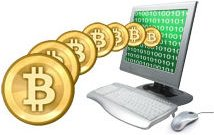
\includegraphics[width=5.00cm]{img/monnaie-electronique.jpg}
\end{minipage}
\footnotetext{\texttt{http://www.numerama.com/magazine/20725-l-hadopi-sonne-la-charge-contre-les-sites-de-streaming-et-de-ddl.html}}

L'Hadopi veut en effet d'abord {\'e}valuer les "\emph{mesures juridiques et techniques existantes et \underline{leurs limites}}", puis se rapprocher des "\emph{interm{\'e}diaires qui contribuent {\`a} leur fonctionnement, dont notamment les {\'e}tablissements bancaires, interm{\'e}diaires de paiement ou de micro-paiement, et r{\'e}gies publicitaires}". Une fois l'action technique au niveau des infrastructures {\'e}cart{\'e}e au vu des nombreuses "limites", ce qui sera le r{\^o}le du Lab R{\'e}seau \& Technique de l'Hadopi, cette derni{\`e}re pourra donc avancer toute la l{\'e}gitimit{\'e} de s'attaquer aux interm{\'e}diaires financiers. ~\\

La m{\'e}thode devrait {\^e}tre simple : ceux qui n'acceptent pas d'embl{\'e}e de couper les vivres aux plateformes de streaming ou de t{\'e}l{\'e}chargement direct seront convoqu{\'e}es au tribunal sur les fondements de l'\texttt{article L336-2 du Code de la Propri{\'e}t{\'e} Intellectuelle~\footnote{\texttt{http://www.legifrance.gouv.fr/affichCodeArticle.do?cidTexte=LEGITEXT000006069414\&idArticle=LEGIARTI000020740350\&dateTexte=20111118}}}, qui dispose que le juge des r{\'e}f{\'e}r{\'e}s peut ordonner "\emph{toutes mesures propres {\`a} pr{\'e}venir ou {\`a} faire cesser une telle atteinte {\`a} un droit d'auteur ou un droit voisin, {\`a} l'encontre de toute personne susceptible de contribuer {\`a} y rem{\'e}dier}". D'une souplesse inouie, cette disposition l{\'e}gislative sera peut-{\^e}tre simplement modifi{\'e}e {\`a} terme, pour permettre {\`a} l'Hadopi elle-m{\^e}me de saisir le tribunal, ce qui est pour le moment une exclusivit{\'e} des ayants droit. ~\\

\textbf{Mais s'attaquer aux flux financiers est-il r{\'e}ellement efficace ?} ~\\

Depuis la lutte judiciaire d{\'e}clench{\'e}e contre Napster il y a plus de dix ans, il est constant que les internautes et les {\'e}diteurs de solutions de partage d'\oe uvres ont toujours su s'adapter {\`a} l'environnement. Ce sont les demandes d'usages qui ont cr{\'e}{\'e} les plateformes de streaming et de t{\'e}l{\'e}chargement ill{\'e}gales, qui aujourd'hui g{\'e}n{\`e}rent des revenus. Si demain les plateformes de streaming et de t{\'e}l{\'e}chargement n'ont plus de ressources pour vivre, elles mourront. Mais les demandes d'usages resteront et seront satisfaites, soit par une offre l{\'e}gale r{\'e}ellement attractive, ce qui reste la cl{\'e} ma{\^i}tresse de la lutte contre le piratage, soit par de nouveaux services invent{\'e}s par "les pirates" pour combler le vide. ~\\

Lorsque l'industrie du disque s'est attaqu{\'e}e {\`a} Kazaa, qui {\'e}tait une soci{\'e}t{\'e} commerciale, les internautes ont cr{\'e}{\'e} et am{\'e}lior{\'e} ensemble eMule et BitTorrent, qui {\'e}taient des solutions P2P open-source sans t{\^e}te contre qui porter plainte. Ils cr{\'e}eront demain des plateformes de streaming et de t{\'e}l{\'e}chargement direct open-source, bas{\'e}es sur des protocoles mieux s{\'e}curis{\'e}s, d{\'e}centralis{\'e}s, qui n'auront pas besoin d'apports d'argent pour vivre. Ces plateformes auront m{\^e}me des avantages nouveaux, comme la possibilit{\'e} d'h{\'e}berger des blogs ou des r{\'e}seaux sociaux non ma{\^i}tris{\'e}s par des soci{\'e}t{\'e}s commerciales, ce que l'on commence {\`a} apercevoir avec la \texttt{Freedom Box~\footnote{\texttt{http://www.numerama.com/magazine/18120-freedombox-liberte-et-vie-privee-offerts-par-un-petit-boitier.html}}}, qui conna{\^i}tra des clones. ~\\

Et si d'aventure les flux financiers restent n{\'e}cessaires, c'est le pire cauchemar des Etats qui risque de se d{\'e}velopper : les monnaies virtuelles. En 2011, \texttt{BitCoin~\footnote{\texttt{http://bitcoin.org/}}} a connu une ascension fulgurante avec une promesse simple, d'{\'e}laboration d'une monnaie de troc qui n'est g{\'e}r{\'e}e par aucun interm{\'e}diaire, exclusivement en P2P. Cet argent ne peut faire l'objet d'aucune imposition, met en danger la souverainet{\'e} de l'Etat, et ne peut pas {\^e}tre r{\'e}gul{\'e}. Les flux financiers ne peuvent pas {\^e}tre bloqu{\'e}s. Le risque n'est pas si th{\'e}orique qu'il peut para{\^i}tre. Si elle peut facilement se d{\'e}velopper dans l'univers num{\'e}rique ("je te vends une application Android en BitCoin, j'ach{\`e}te un acc{\`e}s VPN en Bitcoins), la monnaie virtuelle conna{\^i}t en effet d{\'e}j{\`a} des applications dans les transactions mat{\'e}rielles. Des sites de \texttt{produits bio~\footnote{\texttt{http://www.myhealthyorganics.com/}}}, d'\texttt{aliments pour chiens~\footnote{\texttt{http://www.telepienso.com/}}}, de \texttt{t-shirts~\footnote{\texttt{http://www.squarewear.biz/}}}, de \texttt{parfums~\footnote{\texttt{http://www.shamanscents.com/buy-using-silver-or-bitcoin.html}}}, ou de \texttt{th{\'e}~\footnote{\texttt{http://www.nmteaco.com/bitcoin.html}}} acceptent d{\'e}j{\`a} les BitCoins, qu'ils utilisent pour acheter eux-m{\^e}mes autre chose. Le troc reste le troc, qu'il soit r{\'e}alis{\'e} par l'interm{\'e}diaire d'euros, de dollars, de yuans ou de bitcoins. ~\\

\vfill

\begin{center}
	\begin{minipage}[ht]{6.00cm}
		~\\
	\end{minipage} \hfill \begin{minipage}[ht]{3.00cm}
		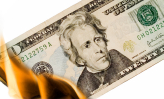
\includegraphics[width=2.75cm]{img/fluxfinanciers.png} 
	\end{minipage} \hfill \begin{minipage}[ht]{3.00cm}
		
\includegraphics[width=2.75cm]{img/bitcoin-vign.png}
	\end{minipage} \hfill \begin{minipage}[ht]{6.00cm}
		~\\
	\end{minipage}
\end{center}

\vfill

\clearpage

\texttt{http://www.lemonde.fr/technologies/article/2013/10/03/silk-road-ferme-et-alors\_3488971\_651865.html}~\\

\textbf{\c{C}a y est, la RIAA s'inqui{\`e}te enfin des Bitcoins}~\\

\emph{\small  Guillaume Champeau -- publi{\'e} le Jeudi 31 Octobre 2013 {\`a} 10h19 -- post{\'e} dans Peer-to-Peer }~\\

\textbf{Alors que la France ne semble toujours pas prendre conscience du danger, le lobby am{\'e}ricain du disque s'inqui{\`e}te de voir The Pirate Bay gagner son ind{\'e}pendance financi{\`e}re avec Bitcoin et Litecoin, deux monnaies virtuelles en P2P qui ne peuvent faire l'objet d'aucune restriction. }~\\

\begin{minipage}[ht]{9.25cm}
	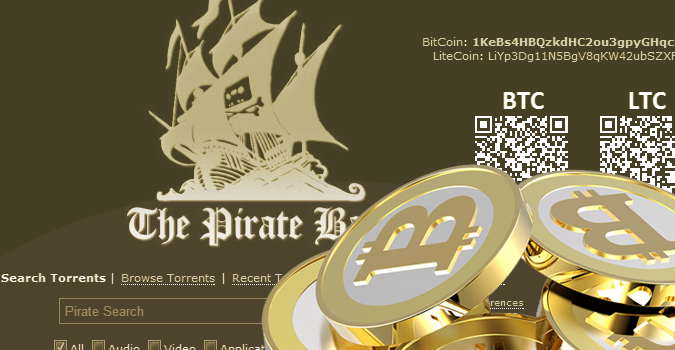
\includegraphics[width=9.00cm]{img/bittorrent-bitcoins.png}
\end{minipage} \hfill \begin{minipage}[ht]{10.00cm}
	D{\`e}s 2011, Numerama avait pr{\'e}venu que les nouvelles tactiques des ayants droits visant {\`a} s'attaquer aux plateformes de paiement et aux r{\'e}gies publicitaires utilis{\'e}es par les sites pirates aurait pour principal effet de donner \texttt{un coup de boost aux monnaies virtuelles en P2P~\footnotemark} comme le Bitcoin ; et que ce serait un probl{\`e}me non seulement pour les ayants droit, mais aussi pour les Etats. Bitcoin pr{\'e}sente en effet la particularit{\'e} de n'{\^e}tre contr{\^o}l{\'e} par aucune puissance {\'e}tatique, de n'avoir aucun interm{\'e}diaire, et de rendre l'argent empoch{\'e} par ses utilisateurs tr{\`e}s difficilement saisissable. Avec les bitcoins, il n'est plus possible de bloquer les flux financiers. ~\\ 
\end{minipage}~\\
\footnotetext{\texttt{http://www.numerama.com/magazine/20727-hadopi-couper-les-flux-financiers-du-piratage-peut-il-vraiment-fonctionner-maj.html}}

Deux ans plus tard, l'industrie musicale commence visiblement {\`a} prendre conscience du probl{\`e}me qui se pr{\'e}sente devant elle -- contrairement au gouvernement qui \texttt{mise sur le gel des moyens financiers~\footnote{\texttt{http://www.numerama.com/magazine/26837-hadopi-des-mesures-anti-piratage-et-pro-filtrage-en-janvier-2014.html}}} des pirates {\`a} travers une mission confi{\'e}e {\`a} la pr{\'e}sidente de la commission de protection des droits de l'Hadopi, et qui n'a donc absolument pas compris que c'{\'e}tait le meilleur moyen de g{\'e}n{\'e}rer une {\'e}conomie alternative hors de contr{\^o}le. ~\\

La Recording Industry Association of America (RIAA), le puissant lobby des grandes maisons de disques, a en effet publi{\'e} \texttt{sa liste des sites pirates~\footnote{\texttt{http://www.scribd.com/doc/180164717/Notorious-Markets-Report-2013-10-25-13-1-pdf}}} qu'elle veut voir dispara{\^i}tre, avec un descriptif d{\'e}taill{\'e} de ses griefs pour chacun d'eux. Or, en {\'e}voquant The Pirate Bay, dont les industries culturelles n'arrive pas {\`a} avoir la peau malgr{\'e} des ann{\'e}es de combat et plusieurs victoires judiciaires, la RIAA s'inqui{\`e}te de l'importance que pourrait prendre les dons en Bitcoins. ~\\

"\emph{En avril 2013, le site a commenc{\'e} {\`a} accepter des dons de la part du public par Bitcoin, une monnaie num{\'e}rique, qui op{\`e}re en utilisant une technologie peer-to-peer}", note la RIAA. "\emph{Il n'y a pas d'autorit{\'e} centrale ou de banque impliqu{\'e}e, ce qui fait qu'il est tr{\`e}s difficile de saisir ou de tracer les fonds Bitcoin. En mai 2013, le site a {\'e}galement commenc{\'e} {\`a} accepter des Litecoin, une autre monnaie internet bas{\'e}e sur le peer-to-peer}". ~\\

Comme le note \texttt{Torrentfreak~\footnote{\texttt{http://torrentfreak.com/riaa-bitcoin-makes-it-hard-to-track-or-seize-pirate-bay-donations-131030/}}}, The Pirate Bay a gagn{\'e} pour le moment pr{\`e}s de 100 Bitcoins r{\'e}partis sur deux comptes, ce qui repr{\'e}sente un peu moins de 15 000 euros (sur Bitcoin, toutes les transactions \texttt{sont publiques~\footnote{\texttt{https://blockchain.info/address/1KeBs4HBQzkdHC2ou3gpyGHqcL7aKzwTve}}}, et anonymes tant que l'internaute ne dit pas publiquement quel est l'identifiant de son compte Bitcoin). 64 Bitcoin re\c{c}us par The Pirate Bay ont ensuite {\'e}t{\'e} utilis{\'e}s, notamment pour soutenir le logiciel de chiffrement \texttt{TrueCrypt~\footnote{\texttt{http://www.truecrypt.org/}}} (9,97 BT). ~\\

\clearpage

\texttt{http://www.01net.com/editorial/607494/bitcoin-la-monnaie-virtuelle-mise-en-danger-par-une-faille-dans-son-protocole/}~\\

\textbf{Bitcoin, la monnaie virtuelle mise en danger par une faille dans son protocole}~\\

\emph{\small \small Pierre Fontaine -- 01net. -- le 07/11/13 {\`a} 20h00  }~\\

\textbf{Alors que le S{\'e}nat am{\'e}ricain s'int{\'e}resse de plus en plus pr{\`e}s aux Bitcoin et que des chercheurs ont trouv{\'e} une faille dans son protocole, la monnaie virtuelle a atteint des sommets de valorisation, d{\'e}montrant un dynamisme impressionnant.} ~\\

Le multivers qu'est Internet est parcouru de milliers de vies et d'anecdotes, contes de f{\'e}e ou cauchemar primal. La vie de Kristoffer Koch se range plut{\^o}t dans la premi{\`e}re cat{\'e}gorie. En 2009, ce jeune Norv{\'e}gien {\'e}tait {\'e}tudiant et r{\'e}digeait sa th{\`e}se sur le chiffrement des informations. Au fil de ses recherches, il {\'e}tait tomb{\'e} sur une cryptomonnaie, alors toute jeune, Bitcoin. Alors, pour voir ce que c'{\'e}tait et parce que l'id{\'e}e lui semblait amusante, Kristoffer Koch a d{\'e}pens{\'e} 150 couronnes, l'{\'e}quivalent d'environ 19 euros d'alors pour acheter des Bitcoin. Puis, il a soutenu sa th{\`e}se, a continu{\'e} sa vie... --- Ces derniers jours, apr{\`e}s une chute du cours li{\'e}s {\`a} divers probl{\`e}mes, autant de r{\'e}putation -- fermeture de Silk Road -- que d'{\'e}cosyst{\`e}me -- d{\'e}clin de MtGox -- le cours du Bitcoin a battu de nouveaux records, apr{\`e}s le boom d'avril dernier, d{\'e}passant les 300 dollars, pour atteindre 235 euros {\`a} son plus haut. A l'heure o{\`u} sont {\'e}crites ses lignes, un Bitcoin s'{\'e}change contre un peu plus de 227 euros. ~\\

\textbf{L'ombre d'une r{\'e}gulation} ~\\

Avec un tel taux de change et une r{\'e}putation de servir {\'e}galement {\`a} financer des transactions ill{\'e}gales, comme c'est le cas sur Silk Road et sa version 2.0, pas {\'e}tonnant que le S{\'e}nat am{\'e}ricain ait d{\'e}cid{\'e} de s'int{\'e}resser de tr{\`e}s pr{\`e}s {\`a} cette monnaie d{\'e}centralis{\'e}e et donc difficilement contr{\^o}lable par un Etat ou une institution. En ao{\^u}t dernier, les autorit{\'e}s am{\'e}ricaines avaient d{\'e}j{\`a} commissionn{\'e}s les agences gouvernementales pour tenter de comprendre ce ph{\'e}nom{\`e}ne. --- Cette fois, deux commissions s{\'e}natoriales, celles de la S{\'e}curit{\'e} nationale et du comit{\'e} bancaire, vont {\'e}tudier les monnaies virtuelles et plus particuli{\`e}rement les Bitcoin afin de voir comment les r{\'e}gulateurs du march{\'e} r{\'e}pondent {\`a} ces nouvelles monnaies. Il sera {\'e}galement question, selon le Wall Street Journal, de voir en quoi ces cryptomonnaies g{\^e}nent la perception de taxes et d'imp{\^o}ts et {\'e}galement leur r{\^o}le dans l'{\'e}conomie parall{\`e}le. ~\\

\begin{minipage}[ht]{8.25cm}
	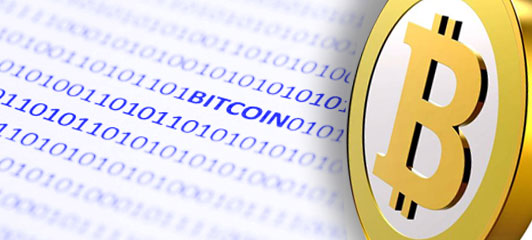
\includegraphics[width=8.00cm]{img/815660.jpg}~\\
\end{minipage} \hfill \begin{minipage}[ht]{11.00cm}
	Cet int{\'e}r{\^e}t insistant pour les Bitcoin montre que les l{\'e}gislateurs entendent faire du dossier Bitcoin une priorit{\'e}. S'il semble impossible qu'ils arrivent {\`a} contr{\^o}ler le fonctionnement m{\^e}me de cette monnaie, ils pourront tenter de mettre des gardes-fous et des verrous sur les terminaisons {\'e}conomiques visibles de cet univers d{\'e}centralis{\'e}. ~\\
\end{minipage}

Les s{\'e}nateurs Carper et Coburn, {\`a} l'origine de cette initiative, indiquait dans une lettre reproduite par le Wall Street Journal que << comme pour toutes les technologies {\'e}mergentes, le gouvernement f{\'e}d{\'e}ral doit s'assurer que les menaces et risques potentiels sont g{\'e}r{\'e}s diligemment >>. << Quoi qu'il en soit, nous devons {\'e}galement {\^e}tre s{\^u}rs que des actions pr{\'e}cipit{\'e}es ou un manque d'information ne vont pas {\'e}touffer une technologie pleine de potentiel >>, pr{\'e}cisaient-ils. Car, c'est bien l{\`a} le risque, confondre Bitcoin et {\'e}conomie souterraine et {\'e}touffer cette monnaie, qui sera remplac{\'e}e par une autre, certes, mais devra retrouver le niveau de confiance et de pr{\'e}sence que semble avoir atteint les Bitcoin aujourd'hui. ~\\

\textbf{L'{\'e}cueil des mineurs {\'e}go{\"i}stes} ~\\

Et justement, le triomphe des Bitcoins, et des cryptomonnaies en g{\'e}n{\'e}ral tiennent en partie dans la confiance li{\'e}e {\`a} la fa\c{c}on dont elles sont g{\'e}n{\'e}r{\'e}es, min{\'e}es. Or, pour deux chercheurs de l'universit{\'e} de Cornell -- Emin Gun Sire, professeur dans cette universit{\'e} et Ittay Eyal, post doc en informatique -- Bitcoin est cass{\'e}, en profondeur. Ils ont publi{\'e} un article, titr{\'e} Majority is not Enough : Bitcoin Mining is Vulnerable, dans lequel ils d{\'e}crivent un moyen d'{\'e}branler le syst{\`e}me de production des Bitcoin. ~\\

En effet, sch{\'e}matiquement, les Bitcoin sont attribu{\'e}s {\`a} la r{\'e}solution de calculs math{\'e}matiques complexes. Chaque << mineur >> touche des Bitcoin en fonction et proportion de sa participation {\`a} la r{\'e}solution de l'{\'e}quation. Or, de plus en plus souvent, afin de lisser leurs revenus en Bitcoin, les mineurs cr{\'e}ent des pools de calcul, et se r{\'e}partissent ensuite les gains. Et justement les chercheurs de Cornell indiquent que de petits pools de mineurs pourraient r{\'e}ussir {\`a} r{\'e}cup{\'e}rer plus de Bitcoin qu'ils n'en << m{\'e}ritent >>. Cette m{\'e}thode est baptis{\'e}e selfish mining  et elle consiste {\`a} cr{\'e}er un fork, une rupture dans la cha{\^i}ne de blocs, qui liste toutes les transactions enregistr{\'e}es -- autrement dit tous les cryptopuzzles r{\'e}solus. Ainsi, un groupe pourraient << miner >> en secret une partie des puzzles sans en avertir le reste de la communaut{\'e}. Il contraindrait ainsi les mineurs ext{\'e}rieurs au groupe {\`a} continuer {\`a} d{\'e}penser de la puissance de calcul sur le puzzle d'origine pendant qu'ils s'attribueraient plus de Bitcoins, en avan\c{c}ant dans la r{\'e}solution de nouveaux cryptopuzzles. ~\\

\begin{minipage}[ht]{9.25cm}
	
\includegraphics[width=9.00cm]{img/815664.jpg}~\\
\end{minipage} \hfill \begin{minipage}[ht]{10.00cm}
	Pire, plus le pool constitu{\'e} par les mineurs peu scrupuleux grossi plus le probl{\`e}me devient important pour l'{\'e}cosyst{\`e}me Bitcoin. Les deux chercheurs ont d{\'e}montr{\'e} qu'avec un peu moins de 10\% de la puissance de calcul total, les mineurs {\'e}go{\"i}stes pourraient {\'e}branl{\'e} le syst{\`e}me entier. Et qu'un groupe qui repr{\'e}senterait 33\% de ce total ne pourrait pas {\^e}tre emp{\^e}ch{\'e} de << miner >> {\'e}go{\"i}stement. ~\\
\end{minipage}

\textbf{Une solution {\`a} d{\'e}ployer} ~\\

Pour autant, ce qui s'apparente {\`a} une attaque du protocole de Bitcoin n'est a priori pas facile {\`a} mettre en place et les deux chercheurs ont propos{\'e} une solution, qui pourrait {\^e}tre int{\'e}gr{\'e}e dans une des mises {\`a} jour du protocole r{\'e}guli{\`e}rement appliqu{\'e}es. Il s'agirait de faire en sorte que les pools de mineurs ne puissent pas poss{\'e}der plus de 25\% du nombre total des n\oe uds constituant le r{\'e}seau, ce qui n'est pas le cas aujourd'hui et peut faciliter ce type de d{\'e}bordement. ~\\

En regard de cette menace potentielle, le hack de inputs.io, porte-monnaie s{\'e}curis{\'e} en ligne pour Bitcoin, para{\^i}t une broutille, m{\^e}me si 4100 Bitcoins ont {\'e}t{\'e} d{\'e}rob{\'e}s. Une belle somme qui a contraint le service attaqu{\'e} {\`a} fermer ses portes. Une preuve suppl{\'e}mentaire de la jeunesse et de la fragilit{\'e} de l'{\'e}cosyst{\`e}me des cryptomonnaies. ~\\

\textbf{Happy end...} ~\\

Mais revenons {\`a} ce cher Kristoffer Koch. --- R{\'e}cemment, entendant parler de Bitcoin, il constate que cela lui rappelle quelque chose. Il se demande alors, certainement en se frappant le front : \emph{<< je n'avais pas un truc du genre ? >>}. Il a ensuite fallu retrouver le mot de passe chiffr{\'e} pour acc{\'e}der {\`a} son compte. Apr{\`e}s quelques vaines tentatives, le s{\'e}same a fini par {\^e}tre retrouv{\'e}. Kristoffer Koch a alors pu acc{\'e}der {\`a} son coffre {\`a} Bitcoin. A l'int{\'e}rieur, si{\'e}geaient les 5 000 Bitcoin qu'il avait achet{\'e}s, le tout repr{\'e}senterait d{\'e}sormais environ 1,075 million d'euros au cours moyen du jour. ~\\

Conscient que les Bitcoin ont encore un certain potentiel, \texttt{Kristoffer Koch~\footnote{\texttt{http://www.01net.com/editorial/606634/monnaie-virtuelle-un-norvegien-soffre-un-appartement-grace-a-ses-bitcoins/}}} n'en a retir{\'e} qu'un cinqui{\`e}me, mille petits Bitcoin, qu'il a transform{\'e} en couronnes norv{\'e}giennes avec lesquels il s'est achet{\'e} un appartement dans un des quartiers les plus hupp{\'e}s d'Oslo. Mais la petite histoire de Kristoffer Koch ne s'arr{\^e}te pas l{\`a}. Sa compagne {\'e}tait pour le moins dubitative, {\`a} l'{\'e}poque, de le voir d{\'e}penser du << vrai argent >> pour acheter du << faux argent >>. Elle lui reprochait souvent d'acheter de ces bricoles inutiles dont les geeks raffolent, l'achat de Bitcoin ayant {\'e}videmment d{\'e}croch{\'e} la timbale de l'achat le plus inconsid{\'e}r{\'e}. Aujourd'hui, dans son appartement de Toyen, {\`a} Oslo, Mme Koch a chang{\'e} d'avis semble-t-il, {\`a} en croire son mari. Maintenant, \emph{<< elle dit que je devrais avoir le droit d'acheter tout ce que je veux... >>}. Une morale qui vaut ce qu'elle vaut, mais ne boudons pas notre plaisir, pour une fois que le gentil, pas {\'e}go{\"i}ste pour un Bitcoin, gagne {\`a} la fin...

\clearpage

\texttt{http://www.01net.com/editorial/591833/bitcoin-la-monnaie-de-geek-qui-vaut-1-milliard-de-dollars/}~\\

\textbf{Bitcoin : la monnaie de geek qui vaut 1 milliard de dollars}~\\

\emph{\small Nathan Sommelier -- 01net. -- le 29/03/13 {\`a} 12h15 }~\\

\begin{minipage}[ht]{9.25cm}
	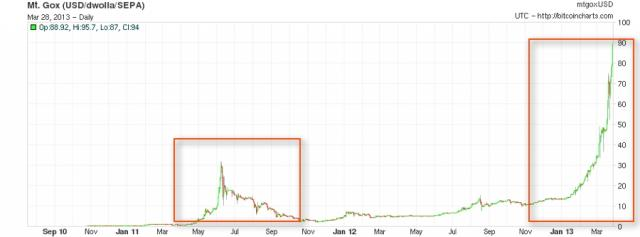
\includegraphics[width=9.00cm]{img/640-755235.jpg}~\\
	\emph{\small L'{\'e}volution du cours du Bitcoin en dollars depuis l'automne 2010. On notera la similitude entre l'explosion du cours en mai-juin 2011 et la hausse ph{\'e}nom{\'e}nale de ce d{\'e}but d'ann{\'e}e. Alors, bulle ou pas bulle ? Une question {\`a} (bient{\^o}t) un milliard de dollars} ~\\
\end{minipage} \hfill \begin{minipage}[ht]{10.00cm}
	\textbf{La hausse vertigineuse de Bitcoin, la d{\'e}sormais c{\'e}l{\`e}bre monnaie virtuelle d{\'e}centralis{\'e}e, lui vaut une attention de plus en plus soutenue de la part des m{\'e}dias et des institutions politiques et financi{\`e}res. Tentative d'explications du ph{\'e}nom{\`e}ne.} ~\\

	Multipli{\'e} par trente. C'est, en l'espace d'un an {\`a} peine, la culbute qu'a connue le cours du Bitcoin. Ce qui fait de cette monnaie d{\'e}mat{\'e}rialis{\'e}e et d{\'e}centralis{\'e}e, comme le soulignait tr{\`e}s r{\'e}cemment le Guardian, la monnaie qui affiche le plus fort taux de croissance au monde, et de loin. Depuis le d{\'e}but de l'ann{\'e}e, le cours du BTC a {\'e}t{\'e} multipli{\'e} par plus de sept. Un Bitcoin vaut aujourd'hui plus de 70 EUR, contre 3 en avril 2012 et 10 environ en janvier 2013.
\end{minipage}

\textbf{L'expansion des usages} ~\\

Il est loin le temps o{\`u} l'usage de Bitcoin comme monnaie d'{\'e}change (et non comme simple valeur sp{\'e}culative ou r{\'e}serve de valeur) {\'e}tait limit{\'e} {\`a} quelques sites de vente clandestine ou de jeu en ligne. Bitcoin est devenu une mani{\`e}re de << voter avec son porte-monnaie >> tout en pr{\'e}servant une composante essentielle du droit de vote : le bulletin secret, et c'est cela m{\^e}me qui lui a valu d'{\^e}tre adopt{\'e} par des ONG ou des organisations comme Wikileaks, ou Wordpress -- afin de permettre aux bloggeurs dissidents ou originaires de pays << exclus >> du syst{\`e}me international de paiements d'acc{\'e}der {\`a} ses services premium. ~\\

\hrule ~\\

{\footnotesize
	\textbf{Bitcoin, c'est quoi ?} ~\\
	
	Bitcoin, cr{\'e}ation d'un personnage {\'e}nigmatique surnomm{\'e} << Satoshi Nakamoto >>, est une devise {\'e}lectronique << virtuelle >>, open-source et d{\'e}centralis{\'e}e, cr{\'e}{\'e}e et s{\'e}curis{\'e}e par un r{\'e}seau peer-to-peer. Gr{\^a}ce {\`a} un syst{\`e}me de validation cryptographique, chaque Bitcoin (BTC) est unique et ne peut {\^e}tre contrefait. ~\\
	
	De plus, la quantit{\'e} totale de BTC qui sera mise en circulation, qui pourra {\^e}tre min{\'e}e (voir encadr{\'e} de bas de page), est volontairement limit{\'e}e {\`a} 21 millions, et prend ainsi le contrepied des politiques inflationnistes des banques centrales. Les BTC sont {\'e}minemment fractionnables et les co{\^u}ts de transaction sont extr{\^e}mement r{\'e}duits compar{\'e}s aux autres syst{\`e}mes de paiement {\'e}lectronique. ~\\
	
	Pour en savoir plus, consultez la page officielle et le Bitcoin Wiki. ~\\
}

\hrule ~\\

Les paiements en Bitcoin, \texttt{accept{\'e}s par des revendeurs de MEGA~\footnote{\texttt{http://www.01net.com/editorial/586919/mega-accepte-les-bitcoins-et-securisera-vos-mails-vos-chats-et-vos-mobiles/}}}, coulent de source pour une soci{\'e}t{\'e} dont le business model s'appuie sur la protection de la vie priv{\'e}e. Mais Bitcoin compte {\'e}galement de nombreux supporters moins sulfureux, comme Archive.org qui accepte les donations en BTC et offre d{\'e}sormais {\`a} ses employ{\'e}s la possibilit{\'e} de recevoir une partie de leur paye en BTC, Namecheap, le revendeur de noms de domaine, ou encore Reddit. ~\\

Gr{\^a}ce aux {\'e}conomies permises par l'utilisation de Bitcoin pour les transactions, le site de vente de produits {\'e}lectroniques Bitcoinstore peut se permettre de pratiquer des prix inf{\'e}rieurs {\`a} ceux des mastodontes de la vente en ligne. Du conseil psychologique {\`a} l'alimentaire en passant par les soins dentaires, un nombre croissant de commerces physiques les acceptent. R{\'e}cemment, un Canadien a m{\^e}me \texttt{mis en vente une propri{\'e}t{\'e} immobili{\`e}re~\footnote{\texttt{http://www.01net.com/editorial/589265/un-canadien-vend-sa-maison-et-son-terrain-contre-des-bitcoins/}}} contre des BTC. ~\\

\clearpage

\textbf{Vers la l{\'e}gitimit{\'e} ?} ~\\

\begin{minipage}[ht]{3.25cm}
	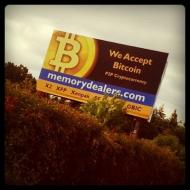
\includegraphics[width=3.00cm]{img/190-755345.jpg}~\\
	\emph{\small Memorydealers, une boutique de la Silicon Valley appartenant aux cr{\'e}ateurs de Bitcoinstore, affiche haut et fort son app{\'e}tit pour la monnaie P2P d{\'e}centralis{\'e}e. } ~\\
\end{minipage} \hfill \begin{minipage}[ht]{16.00cm}
	Bitcoin traverse une {\'e}tape paradoxale de son histoire. La \texttt{soci{\'e}t{\'e} fran\c{c}aise Paymium~\footnotemark} a {\'e}t{\'e} la premi{\`e}re au monde {\`a} cr{\'e}er une bourse de change en Bitcoin en partenariat avec une institution bancaire accr{\'e}dit{\'e}e, offrant ainsi des d{\'e}p{\^o}ts garantis. Les am{\'e}ricains de Coinbase, Coinlab, Tradehill et d'autres lui ont embo{\^i}t{\'e} le pas, soutenus par des fonds de capital-risque. Exante, le premier hedge-fund s'appuyant sur Bitcoin vient de voir le jour {\`a} Malte. ~\\
	
	L'int{\'e}gration de Bitcoin dans le syst{\`e}me financier mondial ne cesse de s'accro{\^i}tre. Le FinCen (l'{\'e}quivalent am{\'e}ricain du Tracfin, l'autorit{\'e} anti-blanchiment) vient d'{\'e}mettre un avis consultatif pr{\'e}conisant la r{\'e}gulation des << {\'e}changeurs >> de monnaies virtuelles, sans toutefois citer directement Bitcoin. Une mesure per\c{c}ue par les << Bitcoiners >> comme une forme de reconnaissance, mais {\'e}galement comme une forme d'attaque indirecte contre la communaut{\'e}, qui pourrait se voir assujettie {\`a} des contraintes draconiennes sur le sol am{\'e}ricain, difficilement compatibles avec l'esprit de Bitcoin. ~\\
\end{minipage}
\footnotetext{\texttt{http://pro.01net.com/editorial/569139/de-nouvelles-pistes-pour-la-monnaie-electronique/}}

L'Europe, pour sa part, reste plus r{\'e}serv{\'e}e. Le porte-parole du commissaire europ{\'e}en Michel Barnier, qui s'{\'e}tait prononc{\'e} sur Bitcoin devant le parlement en 2012, nous a d{\'e}clar{\'e} : << \emph{la valeur mon{\'e}taire des Bitcoins actuellement en circulation} (NDLR : 11 millions de BTC, soit pr{\`e}s d'un milliard de dollars) \emph{reste tr{\`e}s modeste} [...] \emph{et ne n{\'e}cessite pas {\`a} ce stade d'intervention du r{\'e}gulateur. Nous continuerons naturellement {\`a} surveiller l'{\'e}volution de ce march{\'e}, ainsi que les approches adopt{\'e}es par les autres r{\'e}gulateurs.} >> ~\\

\textbf{Caution intellectuelle et engouement populaire} ~\\

Lors d'un colloque sur les syst{\`e}mes de paiement, l'ex-vice-pr{\'e}sident am{\'e}ricain Al Gore s'est fendu d'un << \emph{Je suis fan de Bitcoin} >>. Prenant ouvertement parti pour de nouvelles formes de monnaie apolitiques, il continuait : << \emph{Bitcoin remplace les fonctions du gouvernement par un algorithme... ce qui est plut{\^o}t cool.} [....] \emph{Petit conseil : n'investissez pas dans une usine de porte-monnaie} >>. Pour autant, il soulignait la n{\'e}cessit{\'e} d'un cadre r{\'e}glementaire. Le philosophe, {\'e}crivain et sp{\'e}cialiste du risque financier Nassim Nicholas Taleb d{\'e}clarait il y a quelques jours sur Reddit : << \emph{Bitcoin constitue les pr{\'e}mices de quelque chose de grand : une monnaie sans gouvernement, quelque chose de n{\'e}cessaire et d'imp{\'e}ratif} >>. ~\\

\begin{minipage}[ht]{9.25cm}
	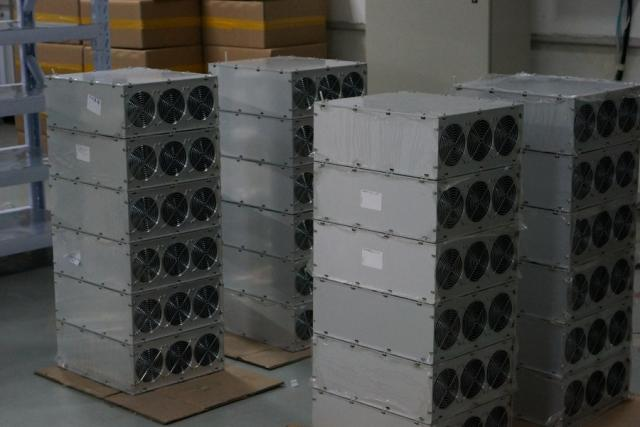
\includegraphics[width=9.00cm]{img/640-755265.jpg}~\\
	\emph{\small Une pile d'unit{\'e}s Avalon chez le fabricant chinois Bitsyncom. Le nouveau visage de la planche {\`a} billets ? L'Avalon ressemble {\`a} une tour de PC mal d{\'e}grossi, mais il s'agit de l'unit{\'e} de calcul de Bitcoins la plus performante disponible sur le march{\'e}. } ~\\
\end{minipage} \hfill \begin{minipage}[ht]{10.00cm}
	Dernier facteur expliquant selon de nombreux observateurs le regain d'int{\'e}r{\^e}t pour Bitcoin : le projet de saisie sur les comptes bancaires chypriotes -- Chypre s'appr{\^e}te d'ailleurs {\`a} accueillir le premier distributeur automatique de Bitcoins -- et la d{\'e}fiance croissante qu'inspire le syst{\`e}me bancaire et la politique mon{\'e}taire des banques centrales, comme en t{\'e}moigne l'explosion r{\'e}cente de t{\'e}l{\'e}chargement d'applications Bitcoin en Espagne, un autre pays durement touch{\'e} par la crise. ~\\
	
	Bitcoin, monnaie d{\'e}mat{\'e}rialis{\'e}e par excellence, serait-il en train de prendre la place des valeurs refuges traditionnelles -- comme les m{\'e}taux pr{\'e}cieux -- en raison de son immunit{\'e} face aux risques de confiscation et au risque souverain ? Entre int{\'e}gration et rejet du syst{\`e}me financier, Bitcoin joue d{\'e}cid{\'e}ment un sacr{\'e} num{\'e}ro d'{\'e}quilibriste... ~\\
\end{minipage}

\hrule ~\\

\clearpage

\textbf{R{\'e}volution chez les mineurs d'or num{\'e}rique} ~\\

\begin{minipage}[ht]{4.25cm}
	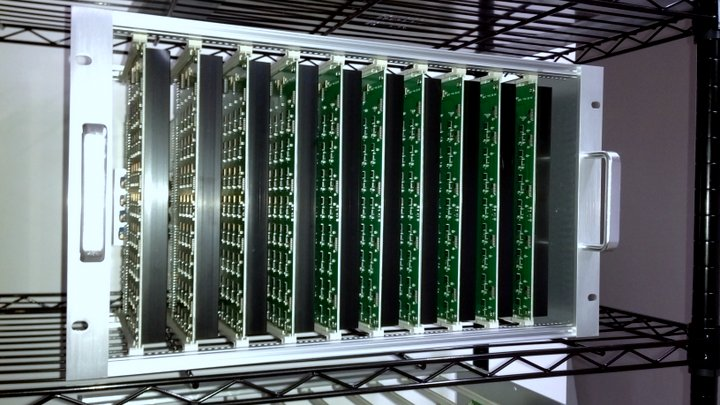
\includegraphics[width=4.00cm]{img/755273.jpg}~\\
\end{minipage} \hfill \begin{minipage}[ht]{15.00cm}
	Bitcoin -- la monnaie -- est cr{\'e}{\'e}e, en dehors de toute autorit{\'e} centralis{\'e}e. Elle est g{\'e}n{\'e}r{\'e}e par les << mineurs >> qui constituent les noeuds de Bitcoin -- le r{\'e}seau d{\'e}centralis{\'e} de validation des transactions -, lesquels apposent leur signature cryptographique en \texttt{r{\'e}solvant des probl{\`e}mes math{\'e}matiques de plus en plus complexes~\footnotemark}. ~\\
\end{minipage}
\footnotetext{\texttt{http://www.e-ducat.fr/economie/dou-vient-la-valeur-des-bitcoins/}}

Les diff{\'e}rents maillons de l'infrastructure indispensable au fonctionnement et {\`a} la p{\'e}rennit{\'e} du r{\'e}seau sont donc r{\'e}compens{\'e}s pour leur participation par la cr{\'e}ation de nouveaux BTC et la r{\'e}partition des frais de transaction, pour l'instant tr{\`e}s modestes. La << difficult{\'e} >> (la complexit{\'e} des op{\'e}rations n{\'e}cessaires pour g{\'e}n{\'e}rer un BTC) augmente avec la puissance totale de calcul du r{\'e}seau. Les mineurs, qui utilisaient {\`a} l'origine de puissantes cartes graphiques, avaient adopt{\'e} en masse les FPGA (puces programmables), bien plus efficaces, l'ann{\'e}e derni{\`e}re. ~\\

Cependant, la donne vient de changer du tout au tout avec l'arriv{\'e}e de puces (ASICs en anglais) d{\'e}di{\'e}es sp{\'e}cialement {\`a} la cr{\'e}ation de Bitcoins. Pour l'instant, seules deux soci{\'e}t{\'e}s sont parvenues {\`a} en produire : le chinois Avalon, qui a vendu des unit{\'e}s au compte-gouttes, et l'am{\'e}ricain ASICMINER, qui vend une participation {\`a} ses << fermes d'ASICs >> sous forme d'actions et reverse des dividendes en BTC. ~\\

Infiniment plus puissants et moins gourmands en {\'e}lectricit{\'e} que tous les {\'e}quipements pr{\'e}c{\'e}dents, les ASICs vont condamner {\`a} l'obsolescence toutes les autres m{\'e}thodes, et faire exploser la puissance totale du r{\'e}seau, et donc la difficult{\'e}. Un facteur interne qui, coupl{\'e} {\`a} la premi{\`e}re division des r{\'e}compenses courant d{\'e}cembre -- les mineurs recevront d{\'e}sormais 25BTC pour le calcul d'un bloc de transactions, au lieu de 50 pr{\'e}c{\'e}demment –, a probablement jou{\'e} un r{\^o}le non n{\'e}gligeable dans la flamb{\'e}e du cours. ~\\

(Ci-contre : Les << racks >> de puces de calcul d'ASICMINER, qui, avec sa puissance calcul et la difficult{\'e} actuelle, g{\'e}n{\`e}re environ 600 BTC par jour, soit plus de 54 000 dollars au cours actuel.) ~\\


\clearpage

\texttt{http://www.bilan.ch/argent-finances-les-plus-de-la-redaction/bitcoin-franchit-la-barre-des-400-dollars}~\\

\textbf{Bitcoin franchit la barre des 400 dollars} --- \emph{\small par Nathan Delaye --- 13 Novembre 2013 }~\\

\textbf{Apr{\`e}s le krach de la monnaie virtuelle en avril, certains observateurs ont craint une bulle. Six mois plus tard, le cours du bitcoin retrouve d{\'e}j{\`a} ses plus hauts sommets. Pourquoi? } ~\\

\begin{minipage}[ht]{9.25cm}
	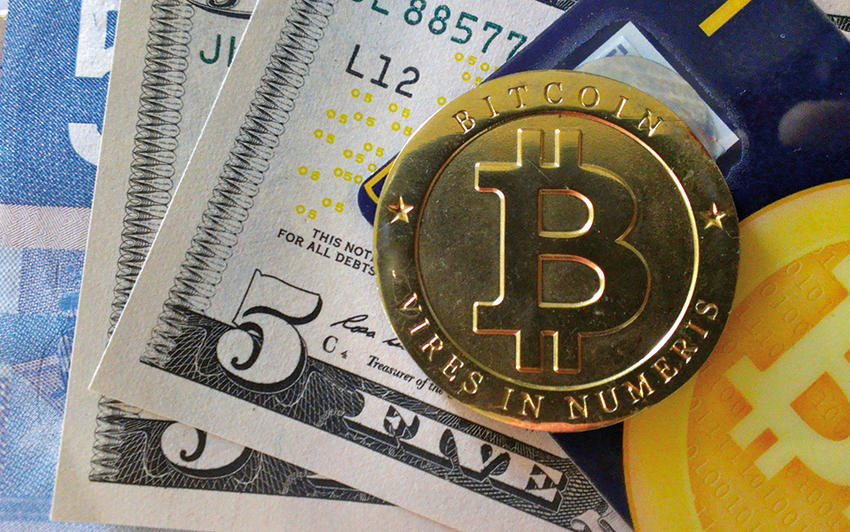
\includegraphics[width=9.00cm]{img/bitcoin_money.jpg}~\\
	\emph{Divisible {\`a} l'infini, le bitcoin a d{\'e}j{\`a} s{\'e}duit 3 millions d'utilisateurs. }~\\
\end{minipage} \hfill \begin{minipage}[ht]{10.00cm}
	\textbf{\textsc{Monnaie}} Apr{\`e}s le krach des dotcoms en 2000, le Nasdaq n'a jamais retrouv{\'e} son niveau. Mais il n'aura fallu que six mois {\`a} la monnaie {\'e}lectronique bitcoin pour effacer les pertes qui ont suivi son krach d'avril dernier et passer la barre des \texttt{400 dollars pour un bitcoin~\footnotemark}. Et cette fois, sans crise chypriote ou autre {\'e}v{\'e}nement financier de nature {\`a} en faire une valeur refuge irrationnelle. ~\\
	
	Ce retour du bitcoin est d'autant plus remarquable qu'entre les attaques des politiciens, comme celle r{\'e}cente du conseiller national socialiste Jean-Christophe Schwaab en Suisse, ou l'arrestation pour blanchiment du fondateur de Silk Road et millionnaire en bitcoins Ross Ulbricht, d{\'e}but octobre {\`a} San Francisco, la monnaie virtuelle sent tellement le soufre que la Tha{\"i}lande l'a interdite. ~\\ 
\end{minipage}~\\
\footnotetext{\texttt{https://www.mtgox.com/}}

Dans ce contexte, comment expliquer que le bitcoin se soit r{\'e}appr{\'e}ci{\'e} si vite? --- Il a des avantages uniques. C'est {\`a} la fois une monnaie universelle et un syst{\`e}me de paiement s{\'e}curis{\'e}, {\'e}changeable contre d'autres devises entre particuliers, de mani{\`e}re anonyme. --- Dans son bureau de Palo Alto, le serial entrepreneur et capital-risqueur Wences Casares conc{\`e}de que la volatilit{\'e} est intrins{\`e}que {\`a} une monnaie qui est <<aujourd'hui un peu comme internet {\`a} l'{\'e}poque de la cr{\'e}ation du premier navigateur>>. Le jeune entrepreneur se dit certain de la tendance haussi{\`e}re du bitcoin. <<Comme l'or, sa quantit{\'e} est limit{\'e}e et aucun Etat ne peut faire pression dessus.>> ~\\

\textbf{Dix fois plus d'utilisateurs} --- Il en veut pour preuve que le ou les inventeurs des cl{\'e}s {\'e}lectroniques du bitcoin, connus sous le pseudonyme de Satoshi Nakamoto, ont disparu. --- <<C'est un signe de plus de la robustesse du syst{\`e}me. Contrairement avec Julian Assange pour WikiLeaks, il n'y a pas de maillon faible dans le bitcoin. Il est d{\'e}j{\`a} r{\'e}parti sur 110 000 serveurs qu'aucun Etat ne pourra interdire globalement>>, poursuit Wences Casares. ~\\

Apr{\`e}s avoir fait fortune en cr{\'e}ant le premier fournisseur d'acc{\`e}s internet d'Argentine puis le premier courtier en ligne d'Am{\'e}rique latine (revendu 800 millions de dollars {\`a} Banco Santander), c'est un observateur int{\'e}ress{\'e} du bitcoin. Lemon, sa derni{\`e}re bo{\^i}te, s'efforce de rendre mobiles les paiements via la monnaie virtuelle. --- Reste que son raisonnement sur l'appr{\'e}ciation programm{\'e}e du bitcoin ne manque pas d'arguments. <<Le nombre d'utilisateurs est pass{\'e} de 300 000 au d{\'e}but de l'ann{\'e}e {\`a} trois millions actuellement. A cause de l'effet r{\'e}seau, il devrait atteindre un milliard dans les cinq ans.>> ~\\

{\'E}tant donn{\'e} que depuis sa cr{\'e}ation, il y a quatre ans, seule la moiti{\'e} des bitcoins possibles sont {\'e}mis (21 millions au total, mais le bitcoin est ind{\'e}finiment divisible), le reste l'{\'e}tant progressivement jusqu'en 2140, son adoption forcerait effectivement son appr{\'e}ciation. Qu'en sera-t-il? ~\\

Immunis{\'e} contre l'inflation et les taxes (sauf en Allemagne qui l'a l{\'e}galis{\'e}), anonyme comme le cash, le bitcoin commence effectivement {\`a} s{\'e}duire l'{\'e}conomie r{\'e}elle (le premier Bancomat vient d'ouvrir {\`a} Vancouver) et m{\^e}me les investisseurs. Wences Casares affirme conserver dans sa banque les bitcoins acquis par des capital-risqueurs mais aussi des g{\'e}rants de hedge funds. --- Eux savent parfaitement que le bitcoin est une exp{\'e}rience {\`a} risque. Mais ils n'oublient pas que, depuis la fin de la libre convertibilit{\'e} du dollar en or en 1971, les banques centrales sont aussi engag{\'e}es dans une exp{\'e}rience mon{\'e}taire in{\'e}dite qui, de krach en quantitave easing, montre qu'elle ne l'est pas forc{\'e}ment moins. ~\\

%% \clearpage

\texttt{http://www.linformaticien.com/actualites/id/31084/les-bitcoins-passent-les-500-dollars-comment-bien-les-utiliser.aspx}~\\

\textbf{Les Bitcoins passent les 500 dollars, comment bien les utiliser ?}

\emph{\small par Emilien Ercolani, le 20 novembre 2013 15:06}~\\

\textbf{Apr{\`e}s le krach de la monnaie virtuelle en avril, certains observateurs ont craint une bulle. Six mois plus tard, le cours du bitcoin retrouve d{\'e}j{\`a} ses plus hauts sommets. Pourquoi? La barre des 500 dollars pour 1 Bitcoin vient d'{\^e}tre franchie. Voici quelques conseils pour bien utiliser les Bitcoins en toute s{\'e}curit{\'e}. } ~\\

L'engouement pour la monnaie virtuelle Bitcoin ne semble pas sur le point de s'essouffler, tant la valeur de celle-ci grimpe de jour en jour. Apr{\`e}s avoir r{\'e}cemment pass{\'e} la barre des 500 dollars l'unit{\'e}, le cours est l{\'e}g{\`e}rement retomb{\'e} mais reste proche de ce cap symbolique alors qu'il avait approch{\'e} les 900 dollars il y a quelques jours ! ~\\ 

Un fait tend {\`a} devenir toutefois in{\'e}luctable : le Bitcoin jouit d'une notori{\'e}t{\'e} croissante {\`a} mesure que le cours grimpe, mais aussi que les m{\'e}dias g{\'e}n{\'e}ralistes s'y int{\'e}ressent. Certains s'interrogent d'ailleurs d{\'e}j{\`a} sur cet {\'e}trange succ{\`e}s et sur son avenir. Son instabilit{\'e} financi{\`e}re est d'ailleurs la source de beaucoup d'articles actuellement. D'autant plus que certaines informations influent fortement sur son cours : lors de la fermeture du supermarch{\'e} de tous les produits illicites sur le Darknet SilkRoad, le cours avait chut{\'e} sous les 100 dollars, pour remonter {\`a} plus de 400 dollars quelques jours apr{\`e}s. ~\\ 

Bref : trop instable, trop fluctuant pour le moment pour que le grand public s'en empare. Toutefois, il n'y aurait rien de surprenant {\`a} ce que vous r{\'e}alisiez votre premi{\`e}re transaction en Bitcoin prochainement. D'o{\`u} quelques r{\`e}gles de s{\'e}curit{\'e} car qui dit monnaie virtuelle dit aussi potentielle menace de s{\'e}curit{\'e}.  ~\\

\textbf{Evitez les banques en ligne} ~\\

C'est l'{\'e}diteur Kaspersky qui livre quelques r{\`e}gles de s{\'e}curit{\'e} basiques si vous utilisez, un jour, des Bitcoins. La premi{\`e}re est simple : ne pas tout placer << \emph{dans une banque en ligne ou sur des plateformes d'{\'e}change en ligne} >>. Ces institutions sont en effet g{\'e}r{\'e}es par des entit{\'e}s anonymes. Aucune garantie donc de r{\'e}cup{\'e}rer votre argent. << \emph{M{\^e}me s'il s'agit d'un {\'e}tablissement r{\'e}put{\'e}, souvenez-vous qu'il existe plus de fa\c{c}ons de p{\'e}n{\'e}trer dans une banque en ligne que dans une chambre forte} >>, rappelle l'{\'e}diteur, qui pr{\'e}cise que c'est moins grave pour des petites sommes d'argent (m{\^e}me si {\`a} 500 dollars le Bitcoin, tout est relatif). ~\\ 

Kaspersky recommande d'utiliser un portefeuille {\'e}lectronique de Bitcoins hors ligne, comme \texttt{Electrum~\footnote{\texttt{http://electrum.org/}}} ou \texttt{Armory~\footnote{\texttt{https://bitcoinarmory.com/}}}. Ces outils vont << \emph{stocker vos bitcoins dans des fichiers compl{\`e}tement chiffr{\'e}s sur votre propre disque dur} >>. En outre, n'oubliez pas d'utiliser un mot de passe fort (id{\'e}alement g{\'e}n{\'e}r{\'e} de mani{\`e}re al{\'e}atoire). Si possible, stockez m{\^e}me votre portefeuille {\'e}lectronique sur un disque dur externe. Nous ne sommes jamais trop prudents.  ~\\

\clearpage

~\\

\clearpage


\end{document}
